\documentclass[10pt,twoside]{article}
\usepackage{./LaTeX/engineeringAssurance}

%Times for rm and math | Helvetica for ss | Courier for tt
\usepackage{mathptmx} % rm & math
\usepackage[scaled=0.90]{helvet} % ss
\usepackage{courier} % tt
\usepackage{amsmath}
\usepackage{enumerate}

\usepackage{alltt}
\normalfont
\usepackage[T1]{fontenc}
\newcommand{\action}[1]{\ensuremath{\langle #1 \rangle}}

\newcommand{\name}[1]{\ensuremath{\textit{#1}}}
\newcommand{\filename}[1]{\ensuremath{\mathtt{#1}}}
\newcommand{\rulespace}{\vspace*{2em}}


\newcommand{\pair}[1]{\ensuremath{\langle #1\rangle}}
%\newcommand{\annd}{\ensuremath{\ \&\ }}
\newcommand{\annd}{\ensuremath{\textrm{ and }}}
% \newcommand{\orr}{\ensuremath{\textrm{ or }}}
\newcommand{\pow}[1]{\ensuremath{\mathcal{P}(#1)}}
\newcommand{\set}[1]{\ensuremath{\{#1\}}}
\newcommand{\midset}[2]{\ensuremath{\set{#1 \mid #2}}}
\newcommand{\arrow}{\ensuremath{\rightarrow}}
\newcommand{\id}[1]{\ensuremath{\textsf{id}_{#1}}}
\newcommand{\subst}[3]{\ensuremath{{#1}\boldsymbol{[}#2\boldsymbol{/}#3\boldsymbol{]}}} 

%% For mathematical proofs with ``reasons'' on each step
\newenvironment{mathprf}
  {\begin{displaymath}\begin{array}{rcll}}{\end{array}\end{displaymath}}
\newcommand{\why}[1]{\ensuremath{\quad \text{#1}}}

%% for conventions (spelled out explicitly in text)
\newenvironment{convention}{\begin{description} \item[\textit{Convention:}
    ]}{\end{description}} 

\newcommand{\readernote}[2]{\noindent\shadowbox{\parbox{.95\textwidth}{%
      \begin{description} \item[\textit{#1:}] #2 \end{description}}}}



\newenvironment{indentedExample}{\begin{example}\ \begin{list}{}{}\item }{\end{list}\end{example}}

%\newenvironment{indentedExample}{\begin{example}}{\end{example}}
% for grammars

\newcommand{\isa}{\ensuremath{\; {:}{:}{=} \;}}
\newcommand{\goesto}{\ensuremath{\leadsto}}
%\newcommand{\ora}{\ensuremath{\;\mid\;}}
\newcommand{\ora}{\ensuremath{\;/\;}}
%\newcommand{\syncat}[1]{\hbox{\textcolor{red}{\sc$\langle$#1$\rangle$}}}
%\newcommand{\syncat}[1]{\hbox{{ \sc$\langle$#1$\rangle$}}}
%\newcommand{\syncat}[1]{\hbox{{ \bf #1 }}}
\newcommand{\syncat}[1]{\ensuremath{\textbf{#1}}\xspace}

% Miscellaneous

\newcommand{\defined}{\ensuremath{\quad \triangleq \quad}}
\newcommand{\defn}{\ensuremath{\stackrel{\mathrm{def}}{=}}}


\newcommand{\assign}{\ensuremath{:=}}

%%% for hiding self comments
%\renewcommand{\suebox}[1]{}
%\renewcommand{\chinbox}[1]{}

\newcommand{\key}[1]{\textbf{#1}}

% encryption

\newcommand{\encrypt}[2]{\ensuremath{\mathit{encrypt}(#2,#1)}}
\newcommand{\cat}[1]{\ensuremath{\langle\!\langle #1 \rangle \! \rangle}}

% Syntactic sets
\newcommand{\PName}{\ensuremath{\textbf{PName}}\xspace}
\newcommand{\PExp}{\ensuremath{\textbf{Princ}}\xspace}
\newcommand{\PropVar}{\ensuremath{\textbf{PropVar}}\xspace}
\newcommand{\LExp}{\ensuremath{\textbf{Form}}\xspace}
\newcommand{\LabelConst}{\ensuremath{\textbf{SecLabel}}\xspace}
\newcommand{\Level}{\ensuremath{\textbf{SecLevel}}\xspace}
\newcommand{\IntLabelConst}{\ensuremath{\textbf{IntLabel}}\xspace}
\newcommand{\IntLevel}{\ensuremath{\textbf{IntLevel}}\xspace}
% \newcommand{\PName}{\ensuremath{\textbf{\textsc{PName}}}\xspace}
% \newcommand{\PExp}{\ensuremath{\textbf{\textsc{Princ}}}\xspace}
% \newcommand{\PropVar}{\ensuremath{\textbf{\textsc{PropVar}}}\xspace}
% \newcommand{\LExp}{\ensuremath{\textbf{\textsc{Form}}}\xspace}
%\newcommand{\LExp}{\ensuremath{\textbf{\underline{Form} }}}
%\newcommand{\privs}{\ensuremath{\mathit{privs}}}
%\newcommand{\Targ}{\ensuremath{\mathcal{T}}}


% Principals
\newcommand{\with}{\ensuremath{\;\&\;}}
\newcommand{\quoting}{\ensuremath{\;|\;}}
\newcommand{\for}[1]{\ensuremath{\;\textsf{for}_{#1}\;}}

% Logical expressions
\newcommand{\has}{\ensuremath{\textsf{ has }}}
\newcommand{\says}{\ensuremath{\text{\footnotesize \textsf{ says }}}}
\newcommand{\controls}{\ensuremath{\text{\footnotesize \textsf{ controls }}}}
\newcommand{\serves}{\ensuremath{\textsf{ serves }}}
\newcommand{\speaksfor}{\ensuremath{\Rightarrow}}
\newcommand{\then}{\;\supset\;}
\newcommand{\phiplus}{\ensuremath{\varphi^{+}}}
% SKC - added syntactic sugar for ``represents''
\newcommand{\rreps}{\ensuremath{\text{\footnotesize \textsf{reps} }}}
\newcommand{\reps}[3]{\ensuremath{{#1} \text{\footnotesize \textsf{
          reps }}{#2}{\text{\footnotesize \textsf{ on }}}{#3}}}
\newcommand{\controlsandsays}{\ensuremath{\textsf{ controls+says }}}
\newcommand{\rp}[2]{\ensuremath{{#1} {\text{\footnotesize \textsf{
          reps }}}{#2}{\text{\footnotesize \textsf{ on }}}}}
\newcommand{\slv}[1]{\ensuremath{\text{\textsf{ slev}}(#1)}}
\newcommand{\ilv}[1]{\ensuremath{\text{\textsf{ ilev}}(#1)}}


% Semantics
\newcommand{\struct}[1]{\ensuremath{\langle {#1} \rangle}}
\newcommand{\krip}[1]{\ensuremath{\langle {#1} \rangle}}

\newcommand{\E}[1]{\ensuremath{\mathcal{E}_{\mathcal{M}}[\![#1]\!]}}
\newcommand{\Ee}{\ensuremath{\mathcal{E}_{\mathcal{M}}}}
\newcommand{\Em}[2]{\ensuremath{\mathcal{E}_{#2}[\![#1]\!]}}

%% for actions: 
%%   \actionit puts contents into textit mode
\newcommand{\action}[1]{\ensuremath{\langle #1 \rangle}}
\newcommand{\actionit}[1]{\ensuremath{\langle \textit{#1} \rangle}}

\newcommand{\sig}[1]{\ensuremath{\mathit{Signature}_{#1}}}

\newcommand{\mssmeet}{\ensuremath{\curlywedge}}
\newcommand{\mssbar}{\ensuremath{\|}}
\newcommand{\below}{\ensuremath{\leq}}

\newcommand{\eqmod}[1]{\ensuremath{\approx_{#1}}}

% Derivability

\newcommand{\infrule}[2]
   {\ensuremath{{\textstyle #1}\over{\textstyle #2}}}

\newcommand{\infname}[1]{\textit{#1}}

\newcommand{\irule}[3]
    {\ensuremath{\infname{#3}\quad {\displaystyle \frac{#1}{#2}}}}

\newcommand{\displaynewrule}[3]
{\begin{displaymath}
  \colorbox{LightGray}{\irule{#1}{#2}{#3}}
%  \colorbox{SpringGreen}{\irule{#1}{#2}{#3}}
\end{displaymath}}

\newcommand{\displaycorerule}[4]
{\begin{displaymath}
  \colorbox{lightgray}{\irule{#1}{#2}{#3}{#4}}
%  \colorbox{SkyBlue}{\irule{#1}{#2}{#3}{#4}}
\end{displaymath}}

\newcommand{\displaycoredef}[1]
{\begin{displaymath}
    \colorbox{lightgray}{\ensuremath{#1}}
%  \colorbox{SkyBlue}{\ensuremath{#1}}
\end{displaymath}}

%% Assorted notation for RBAC
\newcommand{\inherits}{\ensuremath{\,\succeq\,}}   % role inheritance
\newcommand{\Users}{\ensuremath{\mathit{Users}}}
\newcommand{\Perms}{\ensuremath{\mathit{Perms}}}
\newcommand{\Roles}{\ensuremath{\mathit{Roles}}}
\newcommand{\Sessions}{\ensuremath{\mathit{Sessions}}}
\newcommand{\SSD}{\ensuremath{\mathit{SSD}}}
\newcommand{\DSD}{\ensuremath{\mathit{DSD}}}
\newcommand{\ausers}{\ensuremath{\mathit{auth\_users}}}
\newcommand{\aperms}{\ensuremath{\mathit{auth\_perms}}}
\newcommand{\suser}{\ensuremath{\mathit{user}}}
\newcommand{\sroles}{\ensuremath{\mathit{roles}}}


% Generalized addresses
% \newcommand{\genAddr}[2]{\ensuremath{\langle\negmedspace\langle #1
%     \rangle\negmedspace\rangle}{\mid #2}}
\newcommand{\segName}[1]{\ensuremath{\langle\negmedspace\langle #1
    \rangle\negmedspace\rangle}}

%% address-descriptor location for named segment
\newcommand{\adLoc}[1]{\ensuremath{|\!| #1 |\!|}}
\newcommand{\segLoc}[1]
    {\ensuremath{\langle\!\!\langle #1 \rangle\!\!\rangle}}
\newcommand{\genAddr}[2]{\ensuremath{[ #1:#2 ]}}
\newcommand{\genAddrPair}[2]{\ensuremath{(#1,#2)}}

%% Formal proof environment

\newenvironment{formalProof}
{\begin{center}\small\begin{tabular}{ll}}{\end{tabular}\end{center}} 


%% Alternate Formal proof environment



\newenvironment{tabProof}{\begin{center}\footnotesize\begin{tabular}{r
        >{$}p{3.2in}<{$}p{1.0in}}}{\end{tabular}\end{center}}  
\newenvironment{tabProof2}{\begin{center}\footnotesize\begin{tabular}{r >{$}p{2.7in}<{$}p{1.5in}}}{\end{tabular}\end{center}} 

% if then else
\newcommand{\ite}[3]
   {\ensuremath{#1 \rightarrow #2 \mid #3}}

%%  Macro(s) for section summaries
\newcommand*{\summproblem}[1]{\def\fromsummproblem{#1}}
\newcommand*{\summanalysis}[1]{\def\fromsummanalysis{#1}}
\newcommand*{\summresults}[1]{\def\fromsummresults{#1}}

\newcommand{\missing}{\textsc{Missing Component}}
\summproblem{\missing}
\summanalysis{\missing}
\summresults{\missing}

\newcommand{\makesummary}
  {%\section{Summary} 
    \begin{enumerate}
    \item \textsc{What is the problem?}
%      \begin{quote}
%        \it What is the purpose of my thinking?  What precise
%        question am I trying to answer?  Within what point of view am I
%        thinking?
%      \end{quote}
%      \ \\ 

      \fromsummproblem
    \item  \textsc{How am I analyzing the problem?}
%      \begin{quote}
%        \it What am I taking for granted, and what assumptions am
%        I making? What information am I using?  How am I interpreting
%        that information?  What concepts or ideas are central to my
%        thinking? 
%      \end{quote}
%      \ \\ 

      \fromsummanalysis
    \item \textsc{What are the results?}
%      \begin{quote}
%        \it What conclusions am I coming to?  If I accept the
%        conclusions, what are the implications?  What would the
%        consequences be, if I put my thought into action?
%      \end{quote}
%      \ \\ 

      \fromsummresults
    \end{enumerate}

  \summproblem{\missing}
  \summanalysis{\missing}
  \summresults{\missing}
    
}


%----redefine implication as horseshoe instead of arrow--------

\renewcommand{\implies}{\supset}
\newcommand{\believes}{\ensuremath\textsf{ believes }}

%%% Local Variables: 
%%% mode: latex
%%% TeX-master: "book"
%%% End: 

\renewcommand{\infrule}[2]
   {\ensuremath{{\textstyle #1}\over{\textstyle #2}}}

\renewcommand{\infname}[1]{\textit{#1}}
% \renewcommand{\irule}[3]
%     {\ensuremath{\infname{#3}\quad {\displaystyle \frac{#1}{#2}}}}

\ifx\pdfoutput\undefined
\usepackage[dvips]{graphicx}
\else
\usepackage[pdftex]{graphicx}
\usepackage{epstopdf}
\pdfcompresslevel=9
\fi

%Notes in text
\newcommand{\chinbox}[1]{%
  \fbox{\parbox[t]{6.0in}{\textsc{Note to Self:} 
      \begin{center}
        #1
      \end{center}}}}

\newcommand{\problembox}[1]
{
  \fbox{\begin{minipage}{0.9\linewidth}
      \begin{center}
        \redtext{\underline{\textbf{\textsc{Assignment}}}}
      \end{center}
      #1
  \end{minipage}}
}


\usepackage{array}

% ---------------------------------------------------------------------
% Input defined macros and commands
% ---------------------------------------------------------------------
% =====================================================================
%
% Macros for typesetting the HOL system manual
%
% =====================================================================

% ---------------------------------------------------------------------
% Abbreviations for words and phrases
% ---------------------------------------------------------------------

\newcommand\TUTORIAL{{\footnotesize\sl TUTORIAL}}
\newcommand\DESCRIPTION{{\footnotesize\sl DESCRIPTION}}
\newcommand\REFERENCE{{\footnotesize\sl REFERENCE}}
\newcommand\LOGIC{{\footnotesize\sl LOGIC}}
\newcommand\LIBRARIES{{\footnotesize\sl LIBRARIES}}

\newcommand{\bs}{\texttt{\char'134}} % backslash
\newcommand{\lb}{\texttt{\char'173}} % left brace
\newcommand{\rb}{\texttt{\char'175}} % right brace
\newcommand{\td}{\texttt{\char'176}} % tilde
\newcommand{\lt}{\texttt{\char'74}} % less than
\newcommand{\gt}{\texttt{\char'76}} % greater than
\newcommand{\dol}{\texttt{\char'44}} % dollar
% double back quotes ``
\newcommand{\dq}{\texttt{\char'140\char'140}}
%These macros were included by slind:

\newcommand{\holquote}[1]{\dq#1\dq}

\def\HOL{{\small HOL}}
\def\holn{\HOL}  % i.e. hol n(inety-eight), no digits in
                 % macro names is a bit of a pain; deciding to do away
                 % with hol98 nomenclature means that we just want to
                 % write HOL for hol98.
\def\holnversion{Kananaskis-7}
\def\holnsversion{Kananaskis~7} % version with space rather than hyphen
\def\LCF{{\small LCF}}
\def\LCFLSM{{\small LCF{\kern-.2em}{\normalsize\_}{\kern0.1em}LSM}}
\def\PPL{{\small PP}{\kern-.095em}$\lambda$}
\def\PPLAMBDA{{\small PPLAMBDA}}
\def\ML{{\small ML}}
\def\holmake{\texttt{Holmake}}

\newcommand\ie{\mbox{i{.}e{.}}}
\newcommand\eg{\mbox{e{.}g{.}}}
\newcommand\viz{\mbox{viz{.}}}
\newcommand\adhoc{\mbox{\it ad hoc}}
\newcommand\etal{{\it et al.\/}}
\newcommand\etc{\mbox{etc{.}}}

% ---------------------------------------------------------------------
% Simple abbreviations and macros for mathematical typesetting
% ---------------------------------------------------------------------

\newcommand\fun{{\to}}
\newcommand\prd{{\times}}

\newcommand\conj{\ \wedge\ }
\newcommand\disj{\ \vee\ }
\newcommand\imp{ \Rightarrow }
\newcommand\eqv{\ \equiv\ }
\newcommand\cond{\rightarrow}
\newcommand\vbar{\mid}
\newcommand\turn{\ \vdash\ }
\newcommand\hilbert{\varepsilon}
\newcommand\eqdef{\ \equiv\ }

\newcommand\natnums{\mbox{${\sf N}\!\!\!\!{\sf N}$}}
\newcommand\bools{\mbox{${\sf T}\!\!\!\!{\sf T}$}}

\newcommand\p{$\prime$}
\newcommand\f{$\forall$\ }
\newcommand\e{$\exists$\ }

\newcommand\orr{$\vee$\ }
\newcommand\negg{$\neg$\ }

\newcommand\arrr{$\rightarrow$}
\newcommand\hex{$\sharp $}

\newcommand{\uquant}[1]{\forall #1.\ }
\newcommand{\equant}[1]{\exists #1.\ }
\newcommand{\hquant}[1]{\hilbert #1.\ }
\newcommand{\iquant}[1]{\exists ! #1.\ }
\newcommand{\lquant}[1]{\lambda #1.\ }

\newcommand{\leave}[1]{\\[#1]\noindent}
\newcommand\entails{\mbox{\rule{.3mm}{4mm}\rule[2mm]{.2in}{.3mm}}}

% ---------------------------------------------------------------------
% Font-changing commands
% ---------------------------------------------------------------------

\newcommand{\theory}[1]{\hbox{{\small\tt #1}}}
\newcommand{\theoryimp}[1]{\texttt{#1}}

\newcommand{\con}[1]{{\sf #1}}
\newcommand{\rul}[1]{{\tt #1}}
\newcommand{\ty}[1]{\textsl{#1}}

\newcommand{\ml}[1]{\mbox{{\def\_{\char'137}\texttt{#1}}}}
\newcommand{\holtxt}[1]{\ml{#1}}
\newcommand\ms{\tt}
\newcommand{\s}[1]{{\small #1}}

\newcommand{\pin}[1]{{\bf #1}}
\def\m#1{\mbox{\normalsize$#1$}}

% ---------------------------------------------------------------------
% Abbreviations for particular mathematical constants etc.
% ---------------------------------------------------------------------

\newcommand\T{\con{T}}
\newcommand\F{\con{F}}
\newcommand\OneOne{\con{One\_One}}
\newcommand\OntoSubset{\con{Onto\_Subset}}
\newcommand\Onto{\con{Onto}}
\newcommand\TyDef{\con{Type\_Definition}}
\newcommand\Inv{\con{Inv}}
\newcommand\com{\con{o}}
\newcommand\Id{\con{I}}
\newcommand\MkPair{\con{Mk\_Pair}}
\newcommand\IsPair{\con{Is\_Pair}}
\newcommand\Fst{\con{Fst}}
\newcommand\Snd{\con{Snd}}
\newcommand\Suc{\con{Suc}}
\newcommand\Nil{\con{Nil}}
\newcommand\Cons{\con{Cons}}
\newcommand\Hd{\con{Hd}}
\newcommand\Tl{\con{Tl}}
\newcommand\Null{\con{Null}}
\newcommand\ListPrimRec{\con{List\_Prim\_Rec}}


\newcommand\SimpRec{\con{Simp\_Rec}}
\newcommand\SimpRecRel{\con{Simp\_Rec\_Rel}}
\newcommand\SimpRecFun{\con{Simp\_Rec\_Fun}}
\newcommand\PrimRec{\con{Prim\_Rec}}
\newcommand\PrimRecRel{\con{Prim\_Rec\_Rel}}
\newcommand\PrimRecFun{\con{Prim\_Rec\_Fun}}

\newcommand\bool{\ty{bool}}
\newcommand\num{\ty{num}}
\newcommand\ind{\ty{ind}}
\newcommand\lst{\ty{list}}

% ---------------------------------------------------------------------
% \minipagewidth = \textwidth minus 1.02 em
% ---------------------------------------------------------------------

\newlength{\minipagewidth}
\setlength{\minipagewidth}{\textwidth}
\addtolength{\minipagewidth}{-1.02em}

% ---------------------------------------------------------------------
% Environment for the items on the title page of a case study
% ---------------------------------------------------------------------

\newenvironment{inset}[1]{\noindent{\large\bf #1}\begin{list}%
{}{\setlength{\leftmargin}{\parindent}%
\setlength{\topsep}{-.1in}}\item }{\end{list}\vskip .4in}

% ---------------------------------------------------------------------
% Macros for little HOL sessions displayed in boxes.
%
% Usage: (1) \setcounter{sessioncount}{1} resets the session counter
%
%        (2) \begin{session}\begin{verbatim}
%             .
%              < lines from hol session >
%             .
%            \end{verbatim}\end{session}
%
%            typesets the session in a numbered box.
% ---------------------------------------------------------------------

\newlength{\hsbw}
\setlength{\hsbw}{\textwidth}
\addtolength{\hsbw}{-\arrayrulewidth}
\addtolength{\hsbw}{-\tabcolsep}
\newcommand\HOLSpacing{13pt}

\newcounter{sessioncount}
\setcounter{sessioncount}{0}

\newenvironment{session}{\begin{flushleft}
 \refstepcounter{sessioncount}
 \begin{tabular}{@{}|c@{}|@{}}\hline
 \begin{minipage}[b]{\hsbw}
 \vspace*{-.5pt}
 \begin{flushright}
 \rule{0.01in}{.15in}\rule{0.3in}{0.01in}\hspace{-0.35in}
 \raisebox{0.04in}{\makebox[0.3in][c]{\footnotesize\sl \thesessioncount}}
 \end{flushright}
 \vspace*{-.55in}
 \begingroup\small\baselineskip\HOLSpacing}{\endgroup\end{minipage}\\ \hline
 \end{tabular}
 \end{flushleft}}

% ---------------------------------------------------------------------
% Macro for boxed ML functions, etc.
%
% Usage: (1) \begin{holboxed}\begin{verbatim}
%               .
%               < lines giving names and types of mk functions >
%               .
%            \end{verbatim}\end{holboxed}
%
%            typesets the given lines in a box.
%
%            Conventions: lines are left-aligned under the "g" of begin,
%            and used to highlight primary reference for the ml function(s)
%            that appear in the box.
% ---------------------------------------------------------------------

\newenvironment{holboxed}{\begin{flushleft}
  \begin{tabular}{@{}|c@{}|@{}}\hline
  \begin{minipage}[b]{\hsbw}
% \vspace*{-.55in}
  \vspace*{.06in}
  \begingroup\small\baselineskip\HOLSpacing}{\endgroup\end{minipage}\\ \hline
  \end{tabular}
  \end{flushleft}}

% ---------------------------------------------------------------------
% Macro for unboxed ML functions, etc.
%
% Usage: (1) \begin{hol}\begin{verbatim}
%               .
%               < lines giving names and types of mk functions >
%               .
%            \end{verbatim}\end{hol}
%
%            typesets the given lines exactly like {boxed}, except there's
%            no box.
%
%            Conventions: lines are left-aligned under the "g" of begin,
%            and used to display ML code in verbatim, left aligned.
% ---------------------------------------------------------------------

\newenvironment{hol}{\begin{flushleft}
 \begin{tabular}{c@{}@{}}
 \begin{minipage}[b]{\hsbw}
% \vspace*{-.55in}
 \vspace*{.06in}
 \begingroup\small\baselineskip\HOLSpacing}{\endgroup\end{minipage}\\
 \end{tabular}
 \end{flushleft}}

% ---------------------------------------------------------------------
% Emphatic brackets
% ---------------------------------------------------------------------

\newcommand\leb{\lbrack\!\lbrack}
\newcommand\reb{\rbrack\!\rbrack}


% ---------------------------------------------------------------------
% Quotations
% ---------------------------------------------------------------------


%These macros were included by ap; they are used in Chapters 9 and 10
%of the HOL DESCRIPTION

\newcommand{\inds}%standard infinite set
 {\mbox{\rm I}}

\newcommand{\ch}%standard choice function
 {\mbox{\rm ch}}

\newcommand{\den}[1]%denotational brackets
 {[\![#1]\!]}

\newcommand{\two}%standard 2-element set
 {\mbox{\rm 2}}

%macros for pictures in latex

\def\puthrule(#1,#2)#3{\put(#1,#2){\line(1,0){#3}}}
\def\putvrule(#1,#2)#3{\put(#1,#2){\line(0,1){#3}}}
\def\putdot(#1){\put(#1){\circle*{0.2}}}
\def\ignore#1{}
\def\putgrid(#1,#2)(#3,#4){\multiput(#1,#2)(1,0){#3}{\circle*{0.2}}
\multiput(#1,#2)(0,1){#4}{\circle*{0.2}}}

\def\putdevice(#1,#2)#3{\put(#1,#2){\framebox(4,2){\small{\tt #3}}}}
\def\putport(#1,#2)#3{\put(#1,#2){\makebox(4,1){\small{\tt #3}}}}


% =====================================================================
% Macros for typesetting hol reference manual entries
% =====================================================================

% ---------------------------------------------------------------------
% boolean flag for verbose printing of reference manual typesetting
% ---------------------------------------------------------------------

\newif\ifverboseref
\verbosereffalse                          % don't be verbose

% ---------------------------------------------------------------------
% Macro for generating right-hand page running titles.
% ---------------------------------------------------------------------

\makeatletter

\def\mkhead{\futurelet\@t\chsize}
\def\chsize#1.{\ifx a\@t \markright{{\protect\bf #1}}\else
               \ifx b\@t \markright{{\protect\bf #1}}\else
               \ifx c\@t \markright{{\protect\bf #1}}\else
               \ifx d\@t \markright{{\protect\bf #1}}\else
               \ifx e\@t \markright{{\protect\bf #1}}\else
               \ifx f\@t \markright{{\protect\bf #1}}\else
               \ifx g\@t \markright{{\protect\bf #1}}\else
               \ifx h\@t \markright{{\protect\bf #1}}\else
               \ifx i\@t \markright{{\protect\bf #1}}\else
               \ifx j\@t \markright{{\protect\bf #1}}\else
               \ifx k\@t \markright{{\protect\bf #1}}\else
               \ifx l\@t \markright{{\protect\bf #1}}\else
               \ifx m\@t \markright{{\protect\bf #1}}\else
               \ifx n\@t \markright{{\protect\bf #1}}\else
               \ifx o\@t \markright{{\protect\bf #1}}\else
               \ifx p\@t \markright{{\protect\bf #1}}\else
               \ifx q\@t \markright{{\protect\bf #1}}\else
               \ifx r\@t \markright{{\protect\bf #1}}\else
               \ifx s\@t \markright{{\protect\bf #1}}\else
               \ifx t\@t \markright{{\protect\bf #1}}\else
               \ifx u\@t \markright{{\protect\bf #1}}\else
               \ifx v\@t \markright{{\protect\bf #1}}\else
               \ifx w\@t \markright{{\protect\bf #1}}\else
               \ifx z\@t \markright{{\protect\bf #1}}\else
               \ifx y\@t \markright{{\protect\bf #1}}\else
               \ifx z\@t \markright{{\protect\bf #1}}\else
               \markright{{\protect\small\bf #1}}\fi
               \fi\fi\fi\fi\fi\fi\fi\fi\fi\fi\fi\fi\fi\fi\fi
               \fi\fi\fi\fi\fi\fi\fi\fi\fi\fi}

\makeatother

% ---------------------------------------------------------------------
% \DOC{<object>}  : start a manual entry for <object>.
% ---------------------------------------------------------------------

\newcommand{\DOC}[2]%
{\bigskip
 {\ifverboseref{\def\_{\string_}\typeout{Typesetting: #1}}\fi}
 \bgroup\samepage               % ended after \TYPE
 \mkhead #1.
 \begin{flushleft}
 \begin{tabular}{|c|}\hline
 \begin{minipage}{\minipagewidth}
 \bigskip
 {\def\_{\char'137}\LARGE\tt #2}\autoindex{#1@{\tt #1}}
 \bigskip
 \end{minipage}\\ \hline
 \end{tabular}
 \end{flushleft}
 \vskip10pt}

% ---------------------------------------------------------------------
% \setseps = set the spacing parameters for above and below displays
% ---------------------------------------------------------------------
\def\setseps{\partopsep=0mm\topsep=12pt plus2pt minus2pt}

% ---------------------------------------------------------------------
% flag for typesetting SEEALSO list
% ---------------------------------------------------------------------
\newif\ifseealso
\seealsofalse                     % start false.

% ---------------------------------------------------------------------
% \TYPE {<thing>} : {<type>}
% ---------------------------------------------------------------------
\def\TYPE{\noindent}

% ---------------------------------------------------------------------
% Commands for parts of a \DOC:
%    \SYNOPSIS
%    \DESCRIBE
%    \FAILURE
%    \EXAMPLE
%    \USES
%    \SEEALSO
% ---------------------------------------------------------------------

\newcommand\beforeskip{\vspace{12pt plus4pt minus4pt}}

\newcommand{\SYNOPSIS}%
{\beforeskip\leftline{\large\bf Synopsis}\nobreak\noindent}

\newcommand{\DESCRIBE}%
{\beforeskip\leftline{\large\bf Description}\nobreak\noindent}

\newcommand{\FAILURE}%
{\beforeskip\leftline{\large\bf Failure}\nobreak\noindent}

\newcommand{\EXAMPLE}%
{\beforeskip\leftline{\large\bf Example}\nobreak\noindent}

\newcommand{\USES}%
{\beforeskip\leftline{\large\bf Uses}\nobreak\noindent}

\newcommand{\COMMENTS}%
{\beforeskip\leftline{\large\bf Comments}\nobreak\noindent}

\newcommand{\SEEALSO}%
{\beforeskip\seealsotrue\leftline{\large\bf See also}\nobreak\noindent%
\bgroup\raggedright\small\tt\catcode`\_=12}

% ---- added by S-K Chin --------
\newcommand{\IMPLEMENTATION}%
{\beforeskip\leftline{\large\bf Implementation}\nobreak\noindent}


% ---------------------------------------------------------------------
% \ENDDOC = do nothing, but close off the group started by \SEEALSO
% ---------------------------------------------------------------------

\newcommand{\ENDDOC}{\ifseealso \egroup\seealsofalse \else \relax \fi}

% =====================================================================
% Commands for typesetting theorems
% =====================================================================

\makeatletter

% ---------------------------------------------------------------------
% define \@xboxverb<thing>\ENDTHEOREM to mean <thing>\ENDTHEOREM
% ---------------------------------------------------------------------

\begingroup \catcode `|=0 \catcode `[= 1
\catcode`]=2 \catcode `\{=12 \catcode `\}=12
\catcode`\\=12 |gdef|@xboxverb#1\ENDTHEOREM[#1|ENDTHEOREM]
|endgroup

% ---------------------------------------------------------------------
% \bboxverb<thing> = <thing> in a verbatim box 5mm from left margin
% ---------------------------------------------------------------------

\def\@boxverb{\bgroup\leftskip=5mm\parindent\z@
\parfillskip=\@flushglue\parskip\z@
\obeylines\small\tt \catcode``=13 \@noligs \let\do\@makeother \dospecials}

\def\boxverb{\@boxverb \frenchspacing\@vobeyspaces \@xboxverb}

% ---------------------------------------------------------------------
% \ENDTHEOREM just finishes off the group (and kick page if necessary)
% ---------------------------------------------------------------------

\def\ENDTHEOREM{\egroup\filbreak}

% ---------------------------------------------------------------------
% \THEOREM <name> <thy> ... \ENDTHEOREM = typeset a theorem
% ---------------------------------------------------------------------

\def\THEOREM #1 #2 {
 \autoindex{#1@{\tt #1}}
   \vspace{4mm plus2mm minus1mm}
\noindent {\def\_{{\char'137}}\small\tt #1}\quad({\small\tt #2}) \par \boxverb
}

\makeatother

% ---------------------------------------------------------------------
% The theory name \none = italic "none"
% ---------------------------------------------------------------------

\def\none{{\it none}}


\usepackage{url}
\usepackage[line,arrow,frame,matrix]{xy}
\usepackage{./LaTeX/proof}
\usepackage{holtex}
\usepackage{holtexbasic}

% \usepackage[usenames,dvipsnames]{color}
\definecolor{orange}{rgb}{1,0.5,0}
\newcommand{\redtext}[1]{\textcolor{red}{#1}}
\newcommand{\bluetext}[1]{\textcolor{blue}{#1}}
\newcommand{\magtext}[1]{\textcolor{magenta}{#1}}
\newcommand{\greentext}[1]{\textcolor{green}{#1}}
\newcommand{\orangetext}[1]{\textcolor{orange}{#1}}
\newcommand{\standout}[1]{\textcolor{orange}{#1}}

\newcommand{\seq}[2]{\ensuremath{\set{#1} \vdash {#2}}}
\newcommand{\seqs}[2]{\ensuremath{#1 \vdash {#2}}}
\newcommand{\sq}[1]{\ensuremath{\vdash {#1}}}

\newcommand{\goal}[2]{\ensuremath{\set{#1}\;\text{ ?-- }\;{#2}}}
\newcommand{\goals}[2]{\ensuremath{{#1}\;\text{ ?-- }\;{#2}}}
\newcommand{\gls}[1]{\ensuremath{\text{ ?-- }\;{#1}}}

\renewcommand{\irule}[3]
    {\ensuremath{{\displaystyle \frac{#1}{#2}}\quad \infname{#3}}}
\newcommand{\tac}[3]{
  \ensuremath{\begin{tabular}{c}
    {#1}\\\hline\hline{#2}
  \end{tabular}\quad}{#3}}
% HOL theories

\title{\textsc{Command and Control Scenarios in the Access-Control
    Logic and HOL}}

\author{Assigned: Friday 11 November 2011}

\date{Due: 0800 Friday 18 November 2011}

\makeindex

\begin{document}

% ---------------------------------------------------------------------
% Inputs for HOL reports
% ---------------------------------------------------------------------
\newcommand{\HOLcommandDate}{20 August 2016}
\newcommand{\HOLcommandTime}{11:38}
\begin{SaveVerbatim}{HOLcommandDatatypescommands}
\HOLFreeVar{commands} = \HOLConst{MC} \HOLTyOp{missionCommands} \HOLTokenBar{} \HOLConst{WC} \HOLTyOp{weaponCommands}
\end{SaveVerbatim}
\newcommand{\HOLcommandDatatypescommands}{\UseVerbatim{HOLcommandDatatypescommands}}
\begin{SaveVerbatim}{HOLcommandDatatypesmissionCommands}
\HOLFreeVar{missionCommands} = \HOLConst{go} \HOLTokenBar{} \HOLConst{nogo}
\end{SaveVerbatim}
\newcommand{\HOLcommandDatatypesmissionCommands}{\UseVerbatim{HOLcommandDatatypesmissionCommands}}
\begin{SaveVerbatim}{HOLcommandDatatypesweaponCommands}
\HOLFreeVar{weaponCommands} = \HOLConst{launch} \HOLTokenBar{} \HOLConst{abort}
\end{SaveVerbatim}
\newcommand{\HOLcommandDatatypesweaponCommands}{\UseVerbatim{HOLcommandDatatypesweaponCommands}}
\newcommand{\HOLcommandDatatypes}{
\HOLcommandDatatypescommands\HOLcommandDatatypesmissionCommands\HOLcommandDatatypesweaponCommands}

\newcommand{\HOLmissionRolesDate}{20 August 2016}
\newcommand{\HOLmissionRolesTime}{11:38}
\begin{SaveVerbatim}{HOLmissionRolesDatatypesmissionRoles}
\HOLFreeVar{missionRoles} = \HOLConst{BFC} \HOLTokenBar{} \HOLConst{GFC} \HOLTokenBar{} \HOLConst{BFO} \HOLTokenBar{} \HOLConst{GFO}
\end{SaveVerbatim}
\newcommand{\HOLmissionRolesDatatypesmissionRoles}{\UseVerbatim{HOLmissionRolesDatatypesmissionRoles}}
\newcommand{\HOLmissionRolesDatatypes}{
\HOLmissionRolesDatatypesmissionRoles}
\begin{SaveVerbatim}{HOLmissionRolesTheoremsAlternateControlsOneXXthm}
\HOLTokenTurnstile{} (\HOLFreeVar{M}\HOLSymConst{,}\HOLFreeVar{Oi}\HOLSymConst{,}\HOLFreeVar{Os}) \HOLConst{sat} \HOLFreeVar{P} \HOLConst{says} \HOLFreeVar{f} \HOLSymConst{\HOLTokenImp{}}
   (\HOLFreeVar{M}\HOLSymConst{,}\HOLFreeVar{Oi}\HOLSymConst{,}\HOLFreeVar{Os}) \HOLConst{sat} \HOLFreeVar{P} \HOLConst{controls} \HOLFreeVar{f} \HOLConst{andf} \HOLFreeVar{Q} \HOLConst{controls} \HOLFreeVar{f} \HOLSymConst{\HOLTokenImp{}}
   (\HOLFreeVar{M}\HOLSymConst{,}\HOLFreeVar{Oi}\HOLSymConst{,}\HOLFreeVar{Os}) \HOLConst{sat} \HOLFreeVar{f}
\end{SaveVerbatim}
\newcommand{\HOLmissionRolesTheoremsAlternateControlsOneXXthm}{\UseVerbatim{HOLmissionRolesTheoremsAlternateControlsOneXXthm}}
\begin{SaveVerbatim}{HOLmissionRolesTheoremsAlternateControlsTwoXXthm}
\HOLTokenTurnstile{} (\HOLFreeVar{M}\HOLSymConst{,}\HOLFreeVar{Oi}\HOLSymConst{,}\HOLFreeVar{Os}) \HOLConst{sat} \HOLFreeVar{Q} \HOLConst{says} \HOLFreeVar{f} \HOLSymConst{\HOLTokenImp{}}
   (\HOLFreeVar{M}\HOLSymConst{,}\HOLFreeVar{Oi}\HOLSymConst{,}\HOLFreeVar{Os}) \HOLConst{sat} \HOLFreeVar{P} \HOLConst{controls} \HOLFreeVar{f} \HOLConst{andf} \HOLFreeVar{Q} \HOLConst{controls} \HOLFreeVar{f} \HOLSymConst{\HOLTokenImp{}}
   (\HOLFreeVar{M}\HOLSymConst{,}\HOLFreeVar{Oi}\HOLSymConst{,}\HOLFreeVar{Os}) \HOLConst{sat} \HOLFreeVar{f}
\end{SaveVerbatim}
\newcommand{\HOLmissionRolesTheoremsAlternateControlsTwoXXthm}{\UseVerbatim{HOLmissionRolesTheoremsAlternateControlsTwoXXthm}}
\begin{SaveVerbatim}{HOLmissionRolesTheoremsDualControlXXthm}
\HOLTokenTurnstile{} (\HOLFreeVar{M}\HOLSymConst{,}\HOLFreeVar{Oi}\HOLSymConst{,}\HOLFreeVar{Os}) \HOLConst{sat} \HOLFreeVar{P} \HOLConst{says} \HOLFreeVar{s} \HOLSymConst{\HOLTokenImp{}}
   (\HOLFreeVar{M}\HOLSymConst{,}\HOLFreeVar{Oi}\HOLSymConst{,}\HOLFreeVar{Os}) \HOLConst{sat} \HOLFreeVar{Q} \HOLConst{says} \HOLFreeVar{s} \HOLSymConst{\HOLTokenImp{}}
   (\HOLFreeVar{M}\HOLSymConst{,}\HOLFreeVar{Oi}\HOLSymConst{,}\HOLFreeVar{Os}) \HOLConst{sat} \HOLFreeVar{P} \HOLConst{meet} \HOLFreeVar{Q} \HOLConst{controls} \HOLFreeVar{s} \HOLSymConst{\HOLTokenImp{}}
   (\HOLFreeVar{M}\HOLSymConst{,}\HOLFreeVar{Oi}\HOLSymConst{,}\HOLFreeVar{Os}) \HOLConst{sat} \HOLFreeVar{s}
\end{SaveVerbatim}
\newcommand{\HOLmissionRolesTheoremsDualControlXXthm}{\UseVerbatim{HOLmissionRolesTheoremsDualControlXXthm}}
\begin{SaveVerbatim}{HOLmissionRolesTheoremsImpliedControlsSaysXXthm}
\HOLTokenTurnstile{} \HOLSymConst{\HOLTokenForall{}}\HOLBoundVar{Q}.
     (\HOLFreeVar{M}\HOLSymConst{,}\HOLFreeVar{Oi}\HOLSymConst{,}\HOLFreeVar{Os}) \HOLConst{sat} \HOLFreeVar{P} \HOLConst{says} \HOLFreeVar{s\sb{\mathrm{1}}} \HOLSymConst{\HOLTokenImp{}}
     (\HOLFreeVar{M}\HOLSymConst{,}\HOLFreeVar{Oi}\HOLSymConst{,}\HOLFreeVar{Os}) \HOLConst{sat} \HOLFreeVar{P} \HOLConst{controls} \HOLFreeVar{s\sb{\mathrm{1}}} \HOLSymConst{\HOLTokenImp{}}
     (\HOLFreeVar{M}\HOLSymConst{,}\HOLFreeVar{Oi}\HOLSymConst{,}\HOLFreeVar{Os}) \HOLConst{sat} \HOLFreeVar{s\sb{\mathrm{1}}} \HOLConst{impf} \HOLFreeVar{s\sb{\mathrm{2}}} \HOLSymConst{\HOLTokenImp{}}
     (\HOLFreeVar{M}\HOLSymConst{,}\HOLFreeVar{Oi}\HOLSymConst{,}\HOLFreeVar{Os}) \HOLConst{sat} \HOLBoundVar{Q} \HOLConst{says} \HOLFreeVar{s\sb{\mathrm{2}}}
\end{SaveVerbatim}
\newcommand{\HOLmissionRolesTheoremsImpliedControlsSaysXXthm}{\UseVerbatim{HOLmissionRolesTheoremsImpliedControlsSaysXXthm}}
\newcommand{\HOLmissionRolesTheorems}{
\HOLThmTag{missionRoles}{AlternateControls1_thm}\HOLmissionRolesTheoremsAlternateControlsOneXXthm
\HOLThmTag{missionRoles}{AlternateControls2_thm}\HOLmissionRolesTheoremsAlternateControlsTwoXXthm
\HOLThmTag{missionRoles}{DualControl_thm}\HOLmissionRolesTheoremsDualControlXXthm
\HOLThmTag{missionRoles}{ImpliedControlsSays_thm}\HOLmissionRolesTheoremsImpliedControlsSaysXXthm
}

\newcommand{\HOLmissionStaffDate}{20 August 2016}
\newcommand{\HOLmissionStaffTime}{11:38}
\begin{SaveVerbatim}{HOLmissionStaffDatatypesmissionRoleStaff}
\HOLFreeVar{missionRoleStaff} = \HOLConst{Role} \HOLTyOp{missionRoles} \HOLTokenBar{} \HOLConst{Staff} \HOLTyOp{missionStaff}
\end{SaveVerbatim}
\newcommand{\HOLmissionStaffDatatypesmissionRoleStaff}{\UseVerbatim{HOLmissionStaffDatatypesmissionRoleStaff}}
\begin{SaveVerbatim}{HOLmissionStaffDatatypesmissionStaff}
\HOLFreeVar{missionStaff} = \HOLConst{Alice} \HOLTokenBar{} \HOLConst{Bob} \HOLTokenBar{} \HOLConst{Carol} \HOLTokenBar{} \HOLConst{Dan} \HOLTokenBar{} \HOLConst{Weapon}
\end{SaveVerbatim}
\newcommand{\HOLmissionStaffDatatypesmissionStaff}{\UseVerbatim{HOLmissionStaffDatatypesmissionStaff}}
\newcommand{\HOLmissionStaffDatatypes}{
\HOLmissionStaffDatatypesmissionRoleStaff\HOLmissionStaffDatatypesmissionStaff}
\begin{SaveVerbatim}{HOLmissionStaffTheoremsImpliedControlsDelegationXXthm}
\HOLTokenTurnstile{} \HOLSymConst{\HOLTokenForall{}}\HOLBoundVar{R}.
     (\HOLFreeVar{M}\HOLSymConst{,}\HOLFreeVar{Oi}\HOLSymConst{,}\HOLFreeVar{Os}) \HOLConst{sat} \HOLFreeVar{Q} \HOLConst{controls} \HOLFreeVar{f\sb{\mathrm{1}}} \HOLSymConst{\HOLTokenImp{}}
     (\HOLFreeVar{M}\HOLSymConst{,}\HOLFreeVar{Oi}\HOLSymConst{,}\HOLFreeVar{Os}) \HOLConst{sat} \HOLConst{reps} \HOLFreeVar{P} \HOLFreeVar{Q} \HOLFreeVar{f\sb{\mathrm{1}}} \HOLSymConst{\HOLTokenImp{}}
     (\HOLFreeVar{M}\HOLSymConst{,}\HOLFreeVar{Oi}\HOLSymConst{,}\HOLFreeVar{Os}) \HOLConst{sat} \HOLFreeVar{P} \HOLConst{quoting} \HOLFreeVar{Q} \HOLConst{says} \HOLFreeVar{f\sb{\mathrm{1}}} \HOLSymConst{\HOLTokenImp{}}
     (\HOLFreeVar{M}\HOLSymConst{,}\HOLFreeVar{Oi}\HOLSymConst{,}\HOLFreeVar{Os}) \HOLConst{sat} \HOLFreeVar{f\sb{\mathrm{1}}} \HOLConst{impf} \HOLFreeVar{f\sb{\mathrm{2}}} \HOLSymConst{\HOLTokenImp{}}
     (\HOLFreeVar{M}\HOLSymConst{,}\HOLFreeVar{Oi}\HOLSymConst{,}\HOLFreeVar{Os}) \HOLConst{sat} \HOLBoundVar{R} \HOLConst{says} \HOLFreeVar{f\sb{\mathrm{2}}}
\end{SaveVerbatim}
\newcommand{\HOLmissionStaffTheoremsImpliedControlsDelegationXXthm}{\UseVerbatim{HOLmissionStaffTheoremsImpliedControlsDelegationXXthm}}
\newcommand{\HOLmissionStaffTheorems}{
\HOLThmTag{missionStaff}{ImpliedControlsDelegation_thm}\HOLmissionStaffTheoremsImpliedControlsDelegationXXthm
}

\newcommand{\HOLmissionKeysDate}{20 August 2016}
\newcommand{\HOLmissionKeysTime}{11:38}
\begin{SaveVerbatim}{HOLmissionKeysDatatypesmissionCA}
\HOLFreeVar{missionCA} = \HOLConst{JFCA} \HOLTokenBar{} \HOLConst{BFCA} \HOLTokenBar{} \HOLConst{GFCA}
\end{SaveVerbatim}
\newcommand{\HOLmissionKeysDatatypesmissionCA}{\UseVerbatim{HOLmissionKeysDatatypesmissionCA}}
\begin{SaveVerbatim}{HOLmissionKeysDatatypesmissionKey}
\HOLFreeVar{missionKey} = \HOLConst{Kjfca} \HOLTokenBar{} \HOLConst{Kbfca} \HOLTokenBar{} \HOLConst{Kgfca} \HOLTokenBar{} \HOLConst{Kalice} \HOLTokenBar{} \HOLConst{Kbob} \HOLTokenBar{} \HOLConst{Kcarol}
           \HOLTokenBar{} \HOLConst{Kdan}
\end{SaveVerbatim}
\newcommand{\HOLmissionKeysDatatypesmissionKey}{\UseVerbatim{HOLmissionKeysDatatypesmissionKey}}
\begin{SaveVerbatim}{HOLmissionKeysDatatypesmissionPrincipals}
\HOLFreeVar{missionPrincipals} =
    \HOLConst{MRole} \HOLTyOp{missionRoles}
  \HOLTokenBar{} \HOLConst{MStaff} \HOLTyOp{missionStaff}
  \HOLTokenBar{} \HOLConst{MCA} \HOLTyOp{missionCA}
  \HOLTokenBar{} \HOLConst{MKey} \HOLTyOp{missionKey}
\end{SaveVerbatim}
\newcommand{\HOLmissionKeysDatatypesmissionPrincipals}{\UseVerbatim{HOLmissionKeysDatatypesmissionPrincipals}}
\newcommand{\HOLmissionKeysDatatypes}{
\HOLmissionKeysDatatypesmissionCA\HOLmissionKeysDatatypesmissionKey\HOLmissionKeysDatatypesmissionPrincipals}

\newcommand{\HOLmissionCONOPSOneDate}{20 August 2016}
\newcommand{\HOLmissionCONOPSOneTime}{11:38}
\begin{SaveVerbatim}{HOLmissionCONOPSOneTheoremsBFOXXabortXXthm}
\HOLTokenTurnstile{} (\HOLFreeVar{M}\HOLSymConst{,}\HOLFreeVar{Oi}\HOLSymConst{,}\HOLFreeVar{Os}) \HOLConst{sat} \HOLConst{Name} \HOLConst{BFC} \HOLConst{says} \HOLConst{prop} (\HOLConst{MC} \HOLConst{nogo}) \HOLSymConst{\HOLTokenImp{}}
   (\HOLFreeVar{M}\HOLSymConst{,}\HOLFreeVar{Oi}\HOLSymConst{,}\HOLFreeVar{Os}) \HOLConst{sat} \HOLConst{prop} (\HOLConst{MC} \HOLConst{nogo}) \HOLConst{impf} \HOLConst{prop} (\HOLConst{WC} \HOLConst{abort}) \HOLSymConst{\HOLTokenImp{}}
   (\HOLFreeVar{M}\HOLSymConst{,}\HOLFreeVar{Oi}\HOLSymConst{,}\HOLFreeVar{Os}) \HOLConst{sat} \HOLConst{Name} \HOLConst{BFC} \HOLConst{controls} \HOLConst{prop} (\HOLConst{MC} \HOLConst{nogo}) \HOLSymConst{\HOLTokenImp{}}
   (\HOLFreeVar{M}\HOLSymConst{,}\HOLFreeVar{Oi}\HOLSymConst{,}\HOLFreeVar{Os}) \HOLConst{sat} \HOLConst{Name} \HOLConst{BFO} \HOLConst{says} \HOLConst{prop} (\HOLConst{WC} \HOLConst{abort})
\end{SaveVerbatim}
\newcommand{\HOLmissionCONOPSOneTheoremsBFOXXabortXXthm}{\UseVerbatim{HOLmissionCONOPSOneTheoremsBFOXXabortXXthm}}
\begin{SaveVerbatim}{HOLmissionCONOPSOneTheoremsBFOXXlaunchXXthm}
\HOLTokenTurnstile{} (\HOLFreeVar{M}\HOLSymConst{,}\HOLFreeVar{Oi}\HOLSymConst{,}\HOLFreeVar{Os}) \HOLConst{sat} \HOLConst{Name} \HOLConst{BFC} \HOLConst{says} \HOLConst{prop} (\HOLConst{MC} \HOLConst{go}) \HOLSymConst{\HOLTokenImp{}}
   (\HOLFreeVar{M}\HOLSymConst{,}\HOLFreeVar{Oi}\HOLSymConst{,}\HOLFreeVar{Os}) \HOLConst{sat} \HOLConst{prop} (\HOLConst{MC} \HOLConst{go}) \HOLConst{impf} \HOLConst{prop} (\HOLConst{WC} \HOLConst{launch}) \HOLSymConst{\HOLTokenImp{}}
   (\HOLFreeVar{M}\HOLSymConst{,}\HOLFreeVar{Oi}\HOLSymConst{,}\HOLFreeVar{Os}) \HOLConst{sat} \HOLConst{Name} \HOLConst{BFC} \HOLConst{controls} \HOLConst{prop} (\HOLConst{MC} \HOLConst{go}) \HOLSymConst{\HOLTokenImp{}}
   (\HOLFreeVar{M}\HOLSymConst{,}\HOLFreeVar{Oi}\HOLSymConst{,}\HOLFreeVar{Os}) \HOLConst{sat} \HOLConst{Name} \HOLConst{BFO} \HOLConst{says} \HOLConst{prop} (\HOLConst{WC} \HOLConst{launch})
\end{SaveVerbatim}
\newcommand{\HOLmissionCONOPSOneTheoremsBFOXXlaunchXXthm}{\UseVerbatim{HOLmissionCONOPSOneTheoremsBFOXXlaunchXXthm}}
\begin{SaveVerbatim}{HOLmissionCONOPSOneTheoremsBFOXXweaponsXXabortXXthm}
\HOLTokenTurnstile{} (\HOLFreeVar{M}\HOLSymConst{,}\HOLFreeVar{Oi}\HOLSymConst{,}\HOLFreeVar{Os}) \HOLConst{sat} \HOLConst{Name} \HOLConst{BFO} \HOLConst{says} \HOLConst{prop} (\HOLConst{WC} \HOLConst{abort}) \HOLSymConst{\HOLTokenImp{}}
   (\HOLFreeVar{M}\HOLSymConst{,}\HOLFreeVar{Oi}\HOLSymConst{,}\HOLFreeVar{Os}) \HOLConst{sat}
   \HOLConst{Name} \HOLConst{BFO} \HOLConst{controls} \HOLConst{prop} (\HOLConst{WC} \HOLConst{abort}) \HOLConst{andf}
   \HOLConst{Name} \HOLConst{GFO} \HOLConst{controls} \HOLConst{prop} (\HOLConst{WC} \HOLConst{abort}) \HOLSymConst{\HOLTokenImp{}}
   (\HOLFreeVar{M}\HOLSymConst{,}\HOLFreeVar{Oi}\HOLSymConst{,}\HOLFreeVar{Os}) \HOLConst{sat} \HOLConst{prop} (\HOLConst{WC} \HOLConst{abort})
\end{SaveVerbatim}
\newcommand{\HOLmissionCONOPSOneTheoremsBFOXXweaponsXXabortXXthm}{\UseVerbatim{HOLmissionCONOPSOneTheoremsBFOXXweaponsXXabortXXthm}}
\begin{SaveVerbatim}{HOLmissionCONOPSOneTheoremsGFOXXabortXXthm}
\HOLTokenTurnstile{} (\HOLFreeVar{M}\HOLSymConst{,}\HOLFreeVar{Oi}\HOLSymConst{,}\HOLFreeVar{Os}) \HOLConst{sat} \HOLConst{Name} \HOLConst{GFC} \HOLConst{says} \HOLConst{prop} (\HOLConst{MC} \HOLConst{nogo}) \HOLSymConst{\HOLTokenImp{}}
   (\HOLFreeVar{M}\HOLSymConst{,}\HOLFreeVar{Oi}\HOLSymConst{,}\HOLFreeVar{Os}) \HOLConst{sat} \HOLConst{prop} (\HOLConst{MC} \HOLConst{nogo}) \HOLConst{impf} \HOLConst{prop} (\HOLConst{WC} \HOLConst{abort}) \HOLSymConst{\HOLTokenImp{}}
   (\HOLFreeVar{M}\HOLSymConst{,}\HOLFreeVar{Oi}\HOLSymConst{,}\HOLFreeVar{Os}) \HOLConst{sat} \HOLConst{Name} \HOLConst{GFC} \HOLConst{controls} \HOLConst{prop} (\HOLConst{MC} \HOLConst{nogo}) \HOLSymConst{\HOLTokenImp{}}
   (\HOLFreeVar{M}\HOLSymConst{,}\HOLFreeVar{Oi}\HOLSymConst{,}\HOLFreeVar{Os}) \HOLConst{sat} \HOLConst{Name} \HOLConst{GFO} \HOLConst{says} \HOLConst{prop} (\HOLConst{WC} \HOLConst{abort})
\end{SaveVerbatim}
\newcommand{\HOLmissionCONOPSOneTheoremsGFOXXabortXXthm}{\UseVerbatim{HOLmissionCONOPSOneTheoremsGFOXXabortXXthm}}
\begin{SaveVerbatim}{HOLmissionCONOPSOneTheoremsGFOXXlaunchXXthm}
\HOLTokenTurnstile{} (\HOLFreeVar{M}\HOLSymConst{,}\HOLFreeVar{Oi}\HOLSymConst{,}\HOLFreeVar{Os}) \HOLConst{sat} \HOLConst{Name} \HOLConst{GFC} \HOLConst{says} \HOLConst{prop} (\HOLConst{MC} \HOLConst{go}) \HOLSymConst{\HOLTokenImp{}}
   (\HOLFreeVar{M}\HOLSymConst{,}\HOLFreeVar{Oi}\HOLSymConst{,}\HOLFreeVar{Os}) \HOLConst{sat} \HOLConst{prop} (\HOLConst{MC} \HOLConst{go}) \HOLConst{impf} \HOLConst{prop} (\HOLConst{WC} \HOLConst{launch}) \HOLSymConst{\HOLTokenImp{}}
   (\HOLFreeVar{M}\HOLSymConst{,}\HOLFreeVar{Oi}\HOLSymConst{,}\HOLFreeVar{Os}) \HOLConst{sat} \HOLConst{Name} \HOLConst{GFC} \HOLConst{controls} \HOLConst{prop} (\HOLConst{MC} \HOLConst{go}) \HOLSymConst{\HOLTokenImp{}}
   (\HOLFreeVar{M}\HOLSymConst{,}\HOLFreeVar{Oi}\HOLSymConst{,}\HOLFreeVar{Os}) \HOLConst{sat} \HOLConst{Name} \HOLConst{GFO} \HOLConst{says} \HOLConst{prop} (\HOLConst{WC} \HOLConst{launch})
\end{SaveVerbatim}
\newcommand{\HOLmissionCONOPSOneTheoremsGFOXXlaunchXXthm}{\UseVerbatim{HOLmissionCONOPSOneTheoremsGFOXXlaunchXXthm}}
\begin{SaveVerbatim}{HOLmissionCONOPSOneTheoremsGFOXXweaponsXXabortXXthm}
\HOLTokenTurnstile{} (\HOLFreeVar{M}\HOLSymConst{,}\HOLFreeVar{Oi}\HOLSymConst{,}\HOLFreeVar{Os}) \HOLConst{sat} \HOLConst{Name} \HOLConst{GFO} \HOLConst{says} \HOLConst{prop} (\HOLConst{WC} \HOLConst{abort}) \HOLSymConst{\HOLTokenImp{}}
   (\HOLFreeVar{M}\HOLSymConst{,}\HOLFreeVar{Oi}\HOLSymConst{,}\HOLFreeVar{Os}) \HOLConst{sat}
   \HOLConst{Name} \HOLConst{BFO} \HOLConst{controls} \HOLConst{prop} (\HOLConst{WC} \HOLConst{abort}) \HOLConst{andf}
   \HOLConst{Name} \HOLConst{GFO} \HOLConst{controls} \HOLConst{prop} (\HOLConst{WC} \HOLConst{abort}) \HOLSymConst{\HOLTokenImp{}}
   (\HOLFreeVar{M}\HOLSymConst{,}\HOLFreeVar{Oi}\HOLSymConst{,}\HOLFreeVar{Os}) \HOLConst{sat} \HOLConst{prop} (\HOLConst{WC} \HOLConst{abort})
\end{SaveVerbatim}
\newcommand{\HOLmissionCONOPSOneTheoremsGFOXXweaponsXXabortXXthm}{\UseVerbatim{HOLmissionCONOPSOneTheoremsGFOXXweaponsXXabortXXthm}}
\begin{SaveVerbatim}{HOLmissionCONOPSOneTheoremsWeaponsXXlaunchXXthm}
\HOLTokenTurnstile{} (\HOLFreeVar{M}\HOLSymConst{,}\HOLFreeVar{Oi}\HOLSymConst{,}\HOLFreeVar{Os}) \HOLConst{sat} \HOLConst{Name} \HOLConst{GFO} \HOLConst{says} \HOLConst{prop} (\HOLConst{WC} \HOLConst{launch}) \HOLSymConst{\HOLTokenImp{}}
   (\HOLFreeVar{M}\HOLSymConst{,}\HOLFreeVar{Oi}\HOLSymConst{,}\HOLFreeVar{Os}) \HOLConst{sat} \HOLConst{Name} \HOLConst{BFO} \HOLConst{says} \HOLConst{prop} (\HOLConst{WC} \HOLConst{launch}) \HOLSymConst{\HOLTokenImp{}}
   (\HOLFreeVar{M}\HOLSymConst{,}\HOLFreeVar{Oi}\HOLSymConst{,}\HOLFreeVar{Os}) \HOLConst{sat}
   \HOLConst{Name} \HOLConst{BFO} \HOLConst{meet} \HOLConst{Name} \HOLConst{GFO} \HOLConst{controls} \HOLConst{prop} (\HOLConst{WC} \HOLConst{launch}) \HOLSymConst{\HOLTokenImp{}}
   (\HOLFreeVar{M}\HOLSymConst{,}\HOLFreeVar{Oi}\HOLSymConst{,}\HOLFreeVar{Os}) \HOLConst{sat} \HOLConst{prop} (\HOLConst{WC} \HOLConst{launch})
\end{SaveVerbatim}
\newcommand{\HOLmissionCONOPSOneTheoremsWeaponsXXlaunchXXthm}{\UseVerbatim{HOLmissionCONOPSOneTheoremsWeaponsXXlaunchXXthm}}
\newcommand{\HOLmissionCONOPSOneTheorems}{
\HOLThmTag{missionCONOPS1}{BFO_abort_thm}\HOLmissionCONOPSOneTheoremsBFOXXabortXXthm
\HOLThmTag{missionCONOPS1}{BFO_launch_thm}\HOLmissionCONOPSOneTheoremsBFOXXlaunchXXthm
\HOLThmTag{missionCONOPS1}{BFO_weapons_abort_thm}\HOLmissionCONOPSOneTheoremsBFOXXweaponsXXabortXXthm
\HOLThmTag{missionCONOPS1}{GFO_abort_thm}\HOLmissionCONOPSOneTheoremsGFOXXabortXXthm
\HOLThmTag{missionCONOPS1}{GFO_launch_thm}\HOLmissionCONOPSOneTheoremsGFOXXlaunchXXthm
\HOLThmTag{missionCONOPS1}{GFO_weapons_abort_thm}\HOLmissionCONOPSOneTheoremsGFOXXweaponsXXabortXXthm
\HOLThmTag{missionCONOPS1}{Weapons_launch_thm}\HOLmissionCONOPSOneTheoremsWeaponsXXlaunchXXthm
}

\newcommand{\HOLmissionCONOPSTwoDate}{20 August 2016}
\newcommand{\HOLmissionCONOPSTwoTime}{11:38}
\begin{SaveVerbatim}{HOLmissionCONOPSTwoTheoremsBFOXXlaunchXXthmTwo}
\HOLTokenTurnstile{} (\HOLFreeVar{M}\HOLSymConst{,}\HOLFreeVar{Oi}\HOLSymConst{,}\HOLFreeVar{Os}) \HOLConst{sat}
   \HOLConst{reps} (\HOLConst{Name} (\HOLConst{Staff} \HOLConst{Alice})) (\HOLConst{Name} (\HOLConst{Role} \HOLConst{BFC})) (\HOLConst{prop} (\HOLConst{MC} \HOLConst{go})) \HOLSymConst{\HOLTokenImp{}}
   (\HOLFreeVar{M}\HOLSymConst{,}\HOLFreeVar{Oi}\HOLSymConst{,}\HOLFreeVar{Os}) \HOLConst{sat}
   \HOLConst{Name} (\HOLConst{Staff} \HOLConst{Alice}) \HOLConst{quoting} \HOLConst{Name} (\HOLConst{Role} \HOLConst{BFC}) \HOLConst{says}
   \HOLConst{prop} (\HOLConst{MC} \HOLConst{go}) \HOLSymConst{\HOLTokenImp{}}
   (\HOLFreeVar{M}\HOLSymConst{,}\HOLFreeVar{Oi}\HOLSymConst{,}\HOLFreeVar{Os}) \HOLConst{sat} \HOLConst{prop} (\HOLConst{MC} \HOLConst{go}) \HOLConst{impf} \HOLConst{prop} (\HOLConst{WC} \HOLConst{launch}) \HOLSymConst{\HOLTokenImp{}}
   (\HOLFreeVar{M}\HOLSymConst{,}\HOLFreeVar{Oi}\HOLSymConst{,}\HOLFreeVar{Os}) \HOLConst{sat} \HOLConst{Name} (\HOLConst{Role} \HOLConst{BFC}) \HOLConst{controls} \HOLConst{prop} (\HOLConst{MC} \HOLConst{go}) \HOLSymConst{\HOLTokenImp{}}
   (\HOLFreeVar{M}\HOLSymConst{,}\HOLFreeVar{Oi}\HOLSymConst{,}\HOLFreeVar{Os}) \HOLConst{sat}
   \HOLConst{Name} (\HOLConst{Staff} \HOLConst{Carol}) \HOLConst{quoting} \HOLConst{Name} (\HOLConst{Role} \HOLConst{BFO}) \HOLConst{says}
   \HOLConst{prop} (\HOLConst{WC} \HOLConst{launch})
\end{SaveVerbatim}
\newcommand{\HOLmissionCONOPSTwoTheoremsBFOXXlaunchXXthmTwo}{\UseVerbatim{HOLmissionCONOPSTwoTheoremsBFOXXlaunchXXthmTwo}}
\begin{SaveVerbatim}{HOLmissionCONOPSTwoTheoremsGFOXXlaunchXXthmTwo}
\HOLTokenTurnstile{} (\HOLFreeVar{M}\HOLSymConst{,}\HOLFreeVar{Oi}\HOLSymConst{,}\HOLFreeVar{Os}) \HOLConst{sat}
   \HOLConst{reps} (\HOLConst{Name} (\HOLConst{Staff} \HOLConst{Bob})) (\HOLConst{Name} (\HOLConst{Role} \HOLConst{GFC})) (\HOLConst{prop} (\HOLConst{MC} \HOLConst{go})) \HOLSymConst{\HOLTokenImp{}}
   (\HOLFreeVar{M}\HOLSymConst{,}\HOLFreeVar{Oi}\HOLSymConst{,}\HOLFreeVar{Os}) \HOLConst{sat}
   \HOLConst{Name} (\HOLConst{Staff} \HOLConst{Bob}) \HOLConst{quoting} \HOLConst{Name} (\HOLConst{Role} \HOLConst{GFC}) \HOLConst{says} \HOLConst{prop} (\HOLConst{MC} \HOLConst{go}) \HOLSymConst{\HOLTokenImp{}}
   (\HOLFreeVar{M}\HOLSymConst{,}\HOLFreeVar{Oi}\HOLSymConst{,}\HOLFreeVar{Os}) \HOLConst{sat} \HOLConst{prop} (\HOLConst{MC} \HOLConst{go}) \HOLConst{impf} \HOLConst{prop} (\HOLConst{WC} \HOLConst{launch}) \HOLSymConst{\HOLTokenImp{}}
   (\HOLFreeVar{M}\HOLSymConst{,}\HOLFreeVar{Oi}\HOLSymConst{,}\HOLFreeVar{Os}) \HOLConst{sat} \HOLConst{Name} (\HOLConst{Role} \HOLConst{GFC}) \HOLConst{controls} \HOLConst{prop} (\HOLConst{MC} \HOLConst{go}) \HOLSymConst{\HOLTokenImp{}}
   (\HOLFreeVar{M}\HOLSymConst{,}\HOLFreeVar{Oi}\HOLSymConst{,}\HOLFreeVar{Os}) \HOLConst{sat}
   \HOLConst{Name} (\HOLConst{Staff} \HOLConst{Dan}) \HOLConst{quoting} \HOLConst{Name} (\HOLConst{Role} \HOLConst{GFO}) \HOLConst{says}
   \HOLConst{prop} (\HOLConst{WC} \HOLConst{launch})
\end{SaveVerbatim}
\newcommand{\HOLmissionCONOPSTwoTheoremsGFOXXlaunchXXthmTwo}{\UseVerbatim{HOLmissionCONOPSTwoTheoremsGFOXXlaunchXXthmTwo}}
\newcommand{\HOLmissionCONOPSTwoTheorems}{
\HOLThmTag{missionCONOPS2}{BFO_launch_thm2}\HOLmissionCONOPSTwoTheoremsBFOXXlaunchXXthmTwo
\HOLThmTag{missionCONOPS2}{GFO_launch_thm2}\HOLmissionCONOPSTwoTheoremsGFOXXlaunchXXthmTwo
}


\maketitle
\thispagestyle{empty}
\author{}
\maketitle

\begin{abstract}
  This is a problem where you will devise and verify the logic behind
  the command and control for joint authorization using the
  access-control logic and inference rules in HOL. You will deliver a
  complete report detailing your concepts of operations described in
  the access-control logic where each is formally described and
  verified in HOL.
\end{abstract}

\section{Introduction}
\label{sec:introduction}

\subsection{Objectives}
\label{sec:objectives}

Your task this week is to devise and verify using the access-control
logic \cite{ACST} and its implementation in HOL \cite{HOL}, a command
and control CONOPS for \emph{launching} or \emph{aborting} an action
that involves operations in cyberspace. Examples include pure
cyberspace operations such as disabling a specific computer or
network, the release of information damaging to an adversary, to the
kinetic world of launching remotely piloted aircraft and/or releasing
weapons.

The objective of this week's problem is to give you experience in
devising operations and \emph{assuring the logic behind them using
  HOL} within the specific assumptions on recognized authorities,
authenticated commands, certifications, roles, delegations, and
jurisdictions. The benefits of formal verification in HOL (or any
trustworthy computer-assisted reasoning tool) are (1) \emph{assurance}
of logical correctness, (2) \emph{full disclosure} of all definitions
and assumptions, (3) \emph{rapid evaluation, certification, and reuse}
by third parties, (4) \emph{enhanced conceptual unity} due to clarity
and precision, and (5) \emph{enhanced confidence in achieving mission
  objectives} due to assurance.

This sets a new standard for design, verification, and assurance in
cyber operations.  Please take extra care to do the best possible job
as your reports and HOL code for this week's problem will be used as
evidence of how you are able to achieve assurance of cyber operations
with mathematical rigor to external reviewers of our program.

\subsection{Deliverables}
\label{sec:deliverables}

This week you will deliver the following:
\begin{enumerate}
\item A full written report in the format expected in your Cyber
  Engineering Seminar: Cover Page, Executive Summary, Problem
  Statement, Background, Assumptions, Techniques and Tools, Problem
  Solution, Risk Assessment, and Bibliography.
\item Complete verification of your CONOPS in HOL using the
  access-control logic.
\item Your written report will include appendices giving the contents
  of your theories and your source code.
\item You will deliver electronic copies of your source code and
  reports within the \textbf{subdirectory structure I have
    provided}. By so doing, I can check your work by executing
  \texttt{Holmake} in the subdirectory you send me.
\end{enumerate}
You may use the text, figures, tables, and my HOL source code
\textbf{\redtext{with attribution}}. If you collaborated over ideas,
please note that in your report and your source code. Make sure you
include your name on the title page of your report.

\subsection{Problem Statement}
\label{sec:problem}

Our scenario is one that requires the exercise of joint authority in
the midst of an established trust infrastructure.  This is typical of
joint operations or coalition operations.  The specifics of what is
being controlled are unimportant. It could be an MQ-9 Reaper; it could
be the launch of an air-to-ground missile; it could be the launch of a
strategic nuclear ballistic missile; it could be the transfer of
hundreds of millions of dollars between two banks.

Our scenario has two forces operating jointly: \emph{blue forces} and
\emph{gold forces}.  Each force has its own command structure:
\emph{blue command} and \emph{gold command}. The mission for which we
are designing and assuring a cyber command and control (C2)
infrastructure is described below.
\begin{enumerate}
\item \textbf{Oversight and jurisdiction}: blue and gold authorities have joint
  control over a mission involving the \emph{launching} of a weapon.
  Both blue and gold authorities have two mission commands:
  \texttt{go} and \texttt{nogo}. For the mission to proceed, a person
  in the role of blue commander and a person operating in the role
  gold commander must both issue the \texttt{go} command for the mission
  to proceed.
\item \textbf{Operators}: people who are authorized as blue or gold operators
  ultimately issue the command to the weapon under joint control. The
  agreed-upon policy is the same for both blue and gold operators:
  each operator will issue the \texttt{launch} command when he or she
  receives an authenticated \texttt{go} command from their respective
  commander, e.g., the gold operator will issue the \texttt{launch}
  command to the weapon when his/her gold commander issues the
  \texttt{go} command. The corresponding policy holds for the blue
  operator.  Similarly, if the blue or gold operator receives a
  \texttt{nogo} order from their respective commanders, the operator
  will issue an \texttt{abort} command to the weapon.
\item \textbf{Weapon}: the weapon has two commands: \texttt{launch} and
  \texttt{abort}. \texttt{Launch} activates and deploys the
  weapon. \texttt{Abort} puts the weapon in safe mode and returns the
  weapon to its initial standby state. The policy the weapon is
  designed to operate within is this: (1) the weapon can only be
  launched if it receives an authenticated \texttt{launch} command
  from both the blue operator and gold operator, and (2) either the
  blue operator or gold operator can \texttt{abort} the mission
  without the other's \texttt{abort} command.
\end{enumerate}

Your job is to describe blue operator, gold operator, and weapon
operations in terms of \emph{derived inference rules in the
  access-control logic} that are \emph{formally verified in
  HOL}. These operations will include the expected commands received,
\textbf{policies}, assumptions about jurisdiction and authority,
necessary certifications, and trust assumptions.

\section{Background}
\label{sec:background}

Dual control of operations and critical capabilities is often used in
command and control applications such as strategic ballistic missiles
or high-value commercial transactions. In operations depending on
cyber-enabled command and control, integrity of command and control
(C2) is \emph{everything}.  Imagine if operators questioned whether
their weapons would work correctly. Imagine if operators doubted the
integrity or authenticity of the orders they received. Operations
would grind to a halt because no one could believe anything they were
told, nor would they have confidence in any order they issued.

\paragraph{Centers of Gravity, Critical Capabilities, and Critical
  Requirements}

\begin{figure}[t]
  \centering
  \begin{tabular}{cc}
    \begin{minipage}{0.48\linewidth}
      \centering{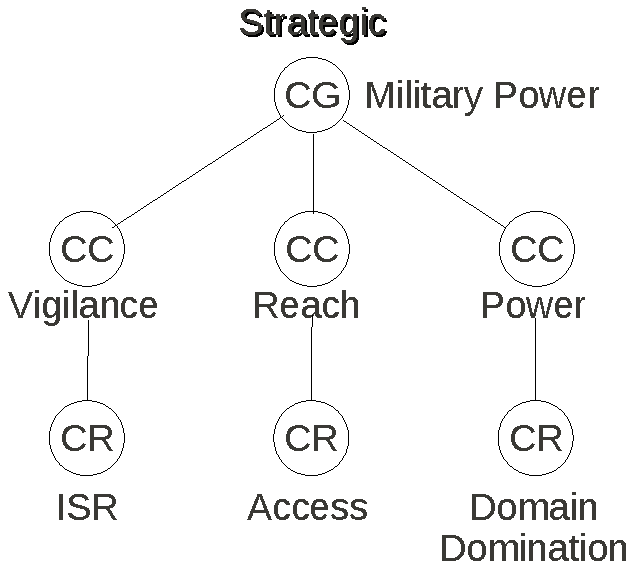
\includegraphics[width=0.6\linewidth]{Figures/milPowerCOG}}
    \end{minipage}
    &
    \begin{minipage}{0.48\linewidth}
     \centering{ 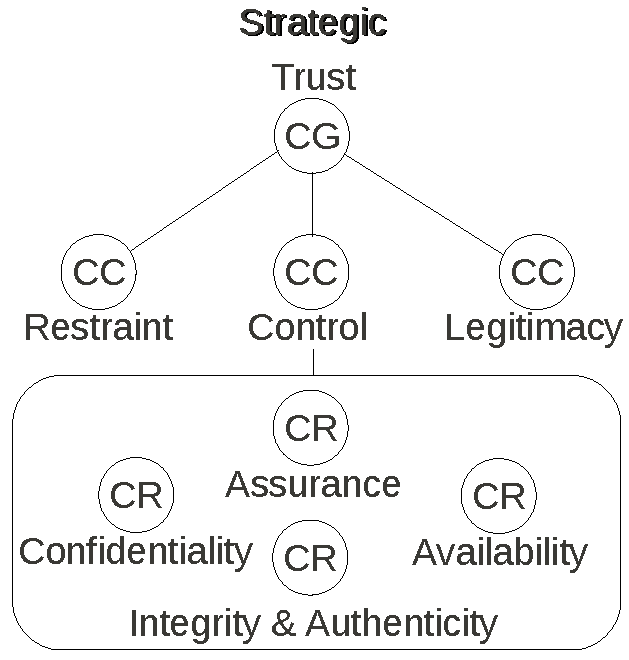
\includegraphics[width=0.6\linewidth]{Figures/trustCOG}}\\
   \end{minipage}\\
   (a) Military Power as a Center of Gravity & (b) Trust as a Center of Gravity\\
  \end{tabular}
  \caption{Military Power and Trust Centers of Gravity}
  \label{fig:cogs}
\end{figure}

Centers of gravity (CGs) are the \emph{primary sources of moral or
  physical strength, power and resistance}.  CGs are \emph{hubs of all
  power}.  In war, a strategic objective is to destroy or neutralize
an adversary's centers of gravity.  By so doing, the adversary is
\emph{dislocated}, i.e., thrown off balance, so that their ability to
operate quickly, decisively, precisely, and correctly is degraded.

Centers of gravity emerge from a collection of primary abilities known
as \textbf{critical capabilities} in the context of a given mission or
scenario.  For example, the combined capabilities of ground, air, and
space surveillance contribute the the critical capability of
\emph{global vigilance} that is one of three critical capabilities
(the others being global reach and global power) that are the basis
for US military as a center of gravity---a hub of US power.

Another center of gravity is \textbf{trust}. Trust and trustworthiness
are crucial at all levels of war and at all levels in
cyberspace. Trust and trustworthiness are both the glue that holds
systems together as well as the oil that keeps systems running
smoothly.  Without trust, systems freeze. In the 2008 financial crisis
that threatened to bankrupt several US banks and financial services
companies, a root cause for the near total disintegration of the
global economy was the fact that loans, risk assessments, property
values, and hence the balance sheets of banks were untrustworthy. When
the lack of trustworthiness of information became apparent, trust
evaporated and the global financial system disintegrated and froze.

In military systems, there are three critical capabilities that
constitute trust as a center of gravity.
\begin{enumerate}
\item Restraint: the ability to exercise appropriate self-control, in
  this case the ability to react with appropriate proportionality,
\item Legitimacy: the acceptance of our actions because of the
  appropriateness of the actions given a particular circumstance,
\item Control: the ability to command and control our forces and
  systems with complete integrity, accuracy, and accountability.
\end{enumerate}
Figure~\ref{fig:cogs}(a) shows military power as a center of gravity
and its critical capabilities and requirements. In an environment
heavily dependent on computer-enabled communications, command and
control, and intelligence (C3I), the trustworthiness of the
computational infrastructure in terms of hardware, software, networks,
and protocols is essential, as is the trustworthiness of the
access control employed from control of physical memory up to and
including information flow policies. Thus, \textbf{trust} as a
strategic center of gravity is alongside military power as a CG.

\paragraph{Assurance of Integrity and Authenticity}

Figure~\ref{fig:cogs}(b) shows trust as a center of gravity along with
the critical capability of \emph{control}. Positive control of forces
requires assurance of confidentiality, availability, and integrity and
authenticity. Again, imagine if operators could not believe the
information or the orders they received. They would be dislocated and
paralyzed. Given the criticality of integrity and authenticity, it is
essential that the highest degree of precision and accuracy of
understanding combined with the highest degree of assurance of
integrity and authenticity be provided to critical missions.  The use
of the access-control logic combined with formal verifications in HOL
enable a rapid, precise, and accurate assessment of the integrity and
authentication CONOPS. As everything is fully disclosed and nothing is
left to the imagination, rapid, precise, and accurate \emph{conceptual
  unity} is achieved.

\section{Assumptions}
\label{sec:assumptions}

Your solutions will be crafted to work in an existing trust
infrastructure that includes:
\begin{enumerate}
\item a hierarchy of certificate authorities to authenticate
  cryptographic keys, provide attribution for messages, and
  authenticate mission roles;
\item the root of trust for cryptographic keys, i.e., the public key
  for the Joint Forces Certificate Authority, $K_{JFCA}$ will be
  distributed in a secure manner to commanders, operators, and weapons
  prior to the mission start;
\item established mission roles in terms of what commands each role
  controls;
\item formally defined mission commands and weapon commands.
\end{enumerate}

\paragraph{Certificate Authority Hierarchy}
\begin{figure}[t]
  \centering
  \begin{tabular}[t]{cc}
    \begin{minipage}{0.48\linewidth}
      % \begin{figure}[t]
      \centering
      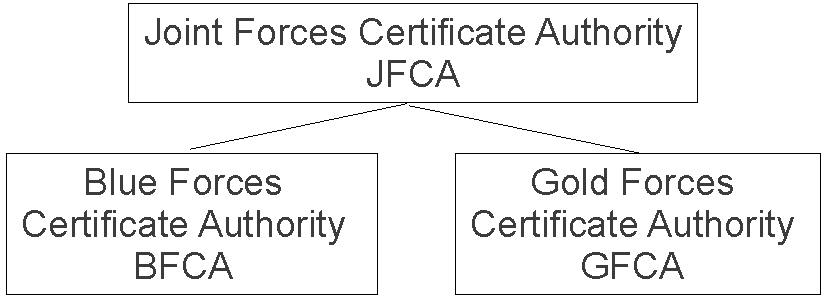
\includegraphics[width=0.95\linewidth]{Figures/CAHierarchy}
      % \caption{Certificate Authority Hierarchy}
      % \label{fig:ca-hierarchy}
      % \end{figure}
    \end{minipage}
    &
    \begin{minipage}{0.48\linewidth}
      % \begin{figure}[t]
      \centering
      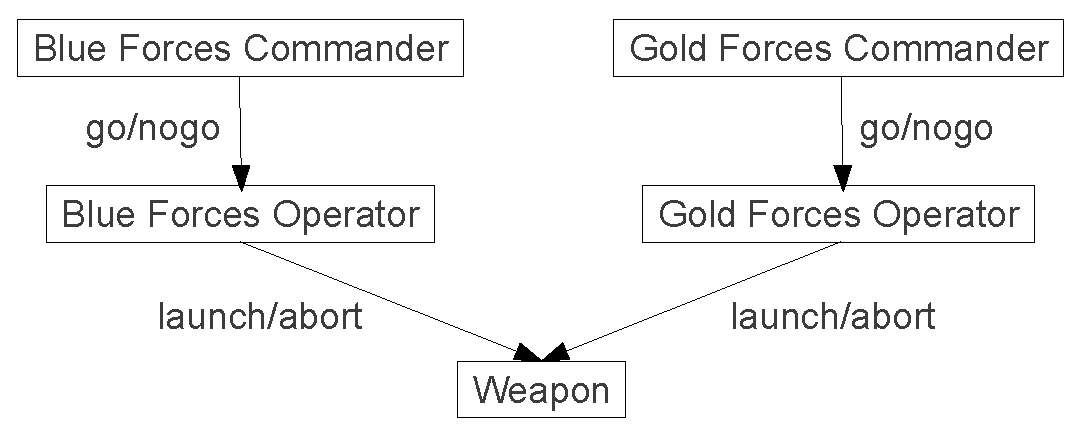
\includegraphics[width=0.95\linewidth]{Figures/conops}
      % \caption{Flow of Command and Control}
      % \label{fig:c2-flow}
      % \end{figure}
    \end{minipage}\\
    (a) Certificate Authority Hierarchy & (b) Flow of Command and Control\\
  \end{tabular}
  
  \caption{Certificate Authority Hierarchy and Flow of Command and Control}
\label{fig:ca-hierarchy-c2-flow}
\end{figure}





Figure~\ref{fig:ca-hierarchy-c2-flow}(a) shows the relationships among the Joint
Forces Certificate Authority (JFCA), Blue Forces Certificate Authority
(BFCA), and Gold Forces Certificate Authority (GFCA).  The primary
purpose of the JFCA is to authenticate the BFCA and GFCA for specific
missions.  Note, it could very well be the case that each joint forces
mission has a different JFCA.  This prevents ``mission creep'' in
terms of authorizations for one mission leaking over to separate
missions.

The BFCA and GFCA are anticipated to be the CAs normally recognized by
Blue and Gold Forces, respectively.  There is no need for cross
recognition of BFCAs or GFCAs independently of the JFCA.  This is
consistent with the intent of establishing JFCAs on a
mission-by-mission basis.

We have the following structure:

\begin{center}
  \begin{tabular}[h]{|r| >{$}c<{$}|l|}
    \hline
    \textbf{Certificate Authority} &\textbf{Associated Key} & \textbf{How Authenticated}\\
    \hline
    JFCA & K_{JFCA} & Pre-distributed to all mission principals\\
    Blue Forces CA & K_{BFCA} & Authenticated by JFCA\\
    Gold Forces CA & K_{GFCA} & Authenticated by JFCA\\
    \hline
  \end{tabular}
\end{center}



\paragraph{Mission Roles and Jurisdiction}

The following mission roles and their authority are stated below.

\begin{center}
  \begin{tabular}[h]{|r| >{$}c<{$}|l|}
    \hline
    \textbf{Role} & \textbf{Controls} & \textbf{How Authenticated}\\
    \hline
    Blue Forces Commander & \texttt{go}/\texttt{nogo} & Pre-distributed to all Blue Forces mission principals\\
    Gold Forces Commander & \texttt{go}/\texttt{nogo} & Pre-distributed to all Gold Forces mission principals\\
    Blue Forces Operator & \texttt{launch}/\texttt{abort} & Blue Forces Commander\\
    Gold Forces Commander & \texttt{launch}/\texttt{abort} & Gold Forces Commander\\
    \hline
  \end{tabular}
\end{center}

\paragraph{Mission Commands and Weapon Commands}
The mission is initiated with a \texttt{go} command; it is aborted
with a \texttt{nogo} command. Mission commands are defined as follows.
\begin{gather*}
  missionCommands \isa go \ora nogo.
\end{gather*}
Weapon commands are defined as follows.
\begin{gather*}
  weaponCommands \isa launch \ora abort.
\end{gather*}
The flow of command and control is shown in Figure~\ref{fig:ca-hierarchy-c2-flow}.

\paragraph{Weapons Policy}

The weapons policy is as follows.
\begin{center}
  \begin{tabular}[h]{|r|l|}
    \hline
    \textbf{Action} & \textbf{Command and Control Requirements}\\
    \hline
    Weapons Launch & \emph{Launch} ordered by both Blue and Gold Operators\\
    Weapons Abort & \emph{Abort} ordered by either Blue or Gold Operator\\
    \hline
  \end{tabular}
\end{center}

% Full technical details for each of the above elements is fully
% disclosed as HOL theories in Section~\ref{sec:techniques-tools}.

\section{Rigorous Representations of Concept of Operations}


\begin{figure}[t]
  \centering
  \begin{tabular}{cc}
    \begin{minipage}{0.48\linewidth}
      \centering{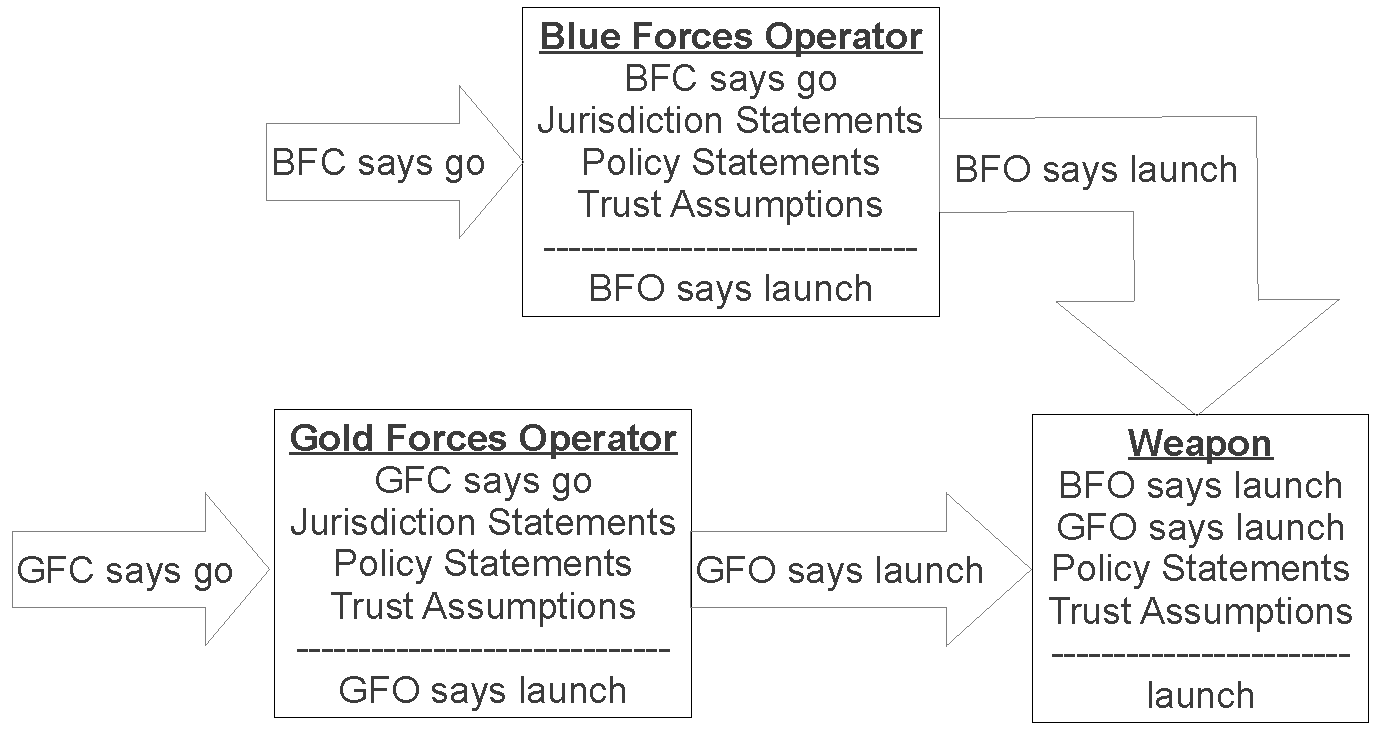
\includegraphics[width=0.95\linewidth]{Figures/launchCONOPS}}
    \end{minipage}
    &
    \begin{minipage}{0.48\linewidth}
      \centering{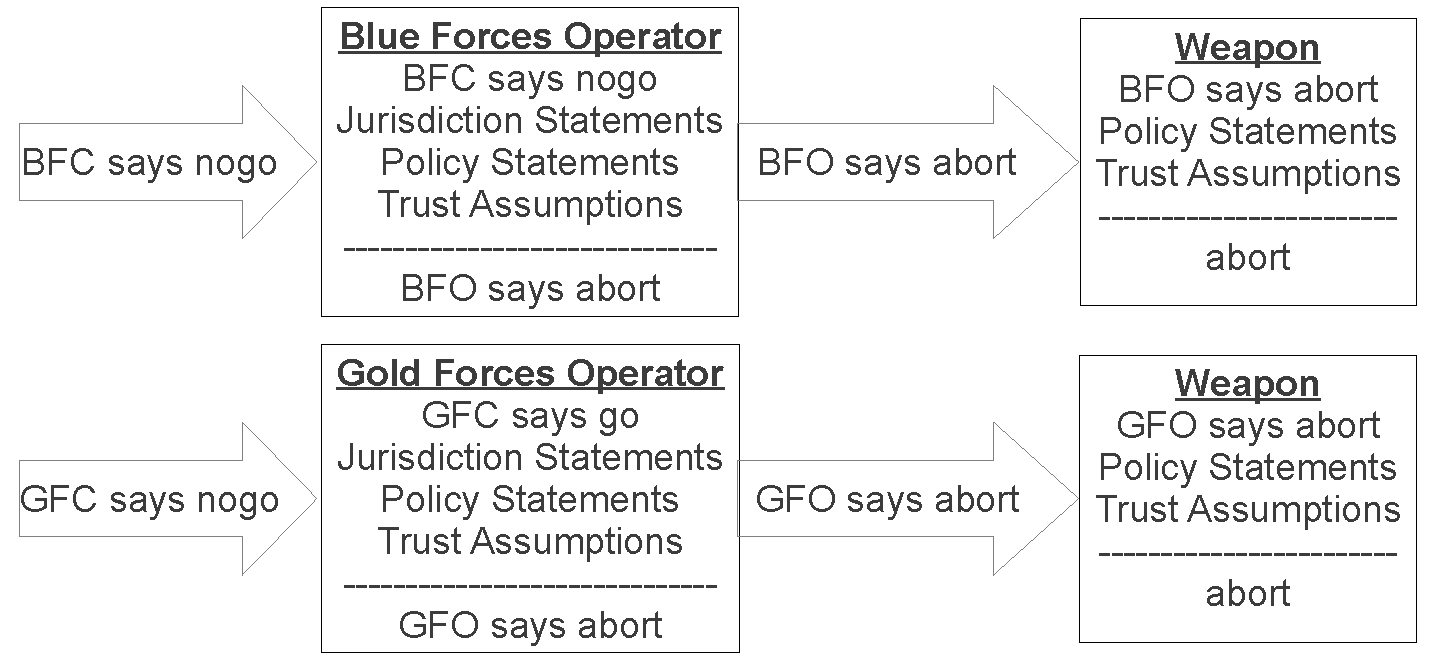
\includegraphics[width=0.95\linewidth]{Figures/abortCONOPS}}
    \end{minipage}\\
    (a) Launch CONOPS & (b) Abort CONOPS\\
  \end{tabular}
  \caption{High-Level View of Launch and Abort CONOPS}
  \label{fig:launch-abort-conops}
\end{figure}

\begin{table}[t]
  \centering
  \begin{tabular}{cc}
  \begin{minipage}{0.4\linewidth}
    \begin{center}
      \begin{tabular}{|r<{.}>{$}l<{$}l|}
        \hline
        1 & P \says \varphi_1 & Received command\\
        2 & P \controls \varphi_1 & Jurisdiction of P\\
        3 & \varphi_1 \implies \varphi_2 & Policy assumption\\
        4 & \varphi_1 & 2, 1 Controls\\
        5 & \varphi_2 & 4, 3 Modus Ponens\\
        6 & Q \says \varphi_2 & 5 Says\\
        \hline
      \end{tabular}
    \end{center}
  \end{minipage}
  &
  \begin{minipage}{0.6\linewidth}
    \begin{center}
      \begin{tabular}{|r<{.}>{$}p{0.45\linewidth}<{$}l|}
        \hline
        1 & P \says \varphi & Received command\\
        2 & Q \says \varphi & Received command\\
        3 & P \with Q \controls \varphi & Dual control policy\\
        4 & (P \says \varphi) \wedge (Q \says \varphi) & 1, 2 Conjunction\\
        5 & (P \says \varphi) \wedge (Q \says \varphi) \equiv P \with Q \says \varphi & \& Says\\
        6 & P \with Q \says \varphi & 5, 4 Equivalence\\
        7 & \varphi & 6, 3 Controls\\
        \hline
      \end{tabular}
    \end{center}

  \end{minipage}\\
  (a) Proof of Implied Controls with Says& (b) Proof of Dual Control
\end{tabular}
  \caption{Proof of Implied Controls with Says Inference Rule}
  \label{tab:implied-controls-with-says-proof}
\end{table}

\begin{table}[t]
  \centering
  \begin{tabular}{cc}
  \begin{minipage}{0.48\linewidth}
    \begin{center}
      \begin{tabular}{|r<{.}>{$}p{0.45\linewidth}<{$}l|}
        \hline
        1 & P \says \varphi & assumption\\
        2 & P \controls \varphi \wedge Q \controls \varphi & assumption\\
        3 & P \controls \varphi & 2 Simplification (1)\\
        4 & \varphi & 2, 1 Controls\\
        \hline
      \end{tabular}
    \end{center}
  \end{minipage}
    &
    \begin{minipage}{0.48\linewidth}
      \begin{center}
        \begin{tabular}{|r<{.}>{$}p{0.45\linewidth}<{$}l|}
          \hline
          1 & Q \says \varphi & assumption\\
          2 & P \controls \varphi \wedge Q \controls \varphi & assumption\\
          3 & Q \controls \varphi & 2 Simplification (2)\\
          4 & \varphi & 2, 1 Controls\\
          \hline
        \end{tabular}
      \end{center}
  \end{minipage}\\
  (a) Proof of Alternate Controls (1) & (b) Proof of Alternate Controls (2)
\end{tabular}
  \caption{Proof of Alternate Controls Rule}
  \label{tab:alternate-controls-proof}
\end{table}

% \subsection{Representing Concepts of Operations in the Access-Control
%   Logic}
% \label{sec:conops}

\begin{center}
  \fbox{\begin{minipage}[h]{0.8\linewidth} Definition of
      \textbf{Concept of Operations}: JP 5-0, Joint Operation Planning
      \begin{small}
        \begin{quote}
          \emph{ ``The CONOPS clearly and concisely expresses what [is
            to be] accomplish[ed] and how it will be done using
            available resources. It describes how the actions of
            $\ldots$ components and supporting organizations will be
            integrated, synchronized, and phased to accomplish the
            mission $\ldots$''}
        \end{quote}
      \end{small}
    \end{minipage}}
\end{center}

Concepts of operations (CONOPS) as stated in the JP 5-0, Joint
Operation Planning definition, describes the coordination,
integration, and sequencing of actions of components and
organizations.  From a command and control standpoint, we focus on the
flow of commands from one principal to the next (recalling that
principals are people, roles, cryptographic keys, processes, etc.),
within a context of policies that govern actions, jurisdiction of
controlling authorities, and trust assumptions.  Using the
access-control logic, each step in a CONOPS---\textbf{a response by a
  principal corresponding to a component in the CONOPS} to a command,
request, or statement in conjunction with policies, jurisdiction of
controlling authorities, and trust assumptions---is a derived
inference rule in the logic. 

Each rule serves as a logical justification of the actions of a CONOPS
component to specific situations. The advantages of using formally
proved inference rules include: (1) establishing the operating
assumptions on which logical validity is based, (2) assurance and full
disclosure due to formal verification, and (3) conceptual unity, when
descriptions and verifications are done and distributed using
computer-assisted reasoning tools such as HOL.

In the three sections that follow, we give three views of the CONOPS
created to satisfy the flow of command and control and certificate
authority hierarchy shown in
Figure~\ref{fig:ca-hierarchy-c2-flow}. Section~\ref{sec:high-level-conops}
gives a high-level description of CONOPS using only the mission roles
of Blue Forces Commander, Blue Forces Operator, Gold Forces Commander,
Gold Forces Operator, and the
Weapon. Section~\ref{sec:conops-with-staff} refines the high-level
CONOPS description by adding people assigned to mission
roles. Section~\ref{sec:conops-with-keys} is the final refinement that
adds cryptographic keys to the flow of control along with certificate
authority hierarchy in Figure~\ref{fig:ca-hierarchy-c2-flow}(a).

\subsection{High-Level CONOPS Description Using Only Mission Roles}
\label{sec:high-level-conops}

Figure~\ref{fig:launch-abort-conops}(a) and (b) show the high-level
CONOPS for launching or aborting the weapon, respectively. Each box
represents a \emph{derived inference rule} in the access-control
logic. The view is high level because the rules are expressed in terms
of roles only.

Notice that the form of Figures~\ref{fig:launch-abort-conops}(a) and
\ref{fig:launch-abort-conops}(b) correspond to the flow of command and
control as shown in Figure~\ref{fig:ca-hierarchy-c2-flow}(b). The
difference is that Figure~\ref{fig:launch-abort-conops} makes all the
hypotheses and conclusions explicit in the form of derived inference
rules. For example, take the box corresponding to \emph{Blue Forces
  Operator}.  \emph{BFO} receives an order from the Blue Forces
Commander: $BFC \says \action{go}$. The Blue Forces Operator evaluates
$BFC \says \action{go}$ in the context of jurisdiction statements,
policy statements, and trust assumptions.  If the Blue Forces Operator
concludes \action{Launch}, then (using the \emph{Says} rule), the Blue
Forces Operator issues the \emph{Launch} command, i.e., $BFO \says
\action{Launch}$.

Essentially, what we must do based on the informal CONOPS statements
and assumptions is write the jurisdiction statements, policy
statements, and trust assumptions necessary for the Blue Forces
Operator to conclude \emph{Launch} when he/she receives the \emph{go}
command from the Blue Forces Commander. 

Perhaps the most straightforward derived inference rule for the Blue
Forces Operator is:
\begin{gather*}
  \irule
  {
    \begin{array}{c}
      BFC \says \action{go} \quad BFC \controls \action{go}\quad
      \action{go} \implies \action{launch}\\
    \end{array}
  }
  {BFO \says \action{launch}}
  {BFO Launch}
\end{gather*}
If the derived inference rule for the Gold Forces Operator has exactly
the same form, i.e.,
\begin{gather*}
  \irule
  {
    \begin{array}{c}
      GFC \says \action{go} \quad GFC \controls \action{go}\quad
      \action{go} \implies \action{launch}\\
    \end{array}
  }
  {GFO \says \action{launch}}
  {GFO Launch},
\end{gather*}
then both Blue and Gold Operators are relying a general inference rule:
\begin{gather*}
  \irule
  {
    \begin{array}{c}
      P \says \varphi_1 \quad P \controls \varphi_1\quad
      \varphi_1 \implies \varphi_2\\
    \end{array}
  }
  {Q \says \varphi_2}
  {Implied Controls with Says}.
\end{gather*}
The proof of the \emph{Implied Controls with Says} inference rule is
shown in Table~\ref{tab:implied-controls-with-says-proof}.
Discovering common logical principles and rules is an advantage
intrinsic to using symbolic logic in general, as well as the
access-control logic in particular.

Turning to the derived inference rule corresponding to the weapon, we
have the following inference rule:
\begin{gather*}
  \irule
  {
    \begin{array}[h]{c}
      P \says \varphi \quad Q \says \varphi \quad P \with Q \controls \varphi
    \end{array}
  }
  {\varphi}
  {Dual Control}
\end{gather*}
The proof of \emph{Dual Control} is given in
Table~\ref{tab:implied-controls-with-says-proof}(b).

Finally, we turn to the high-level abort CONOPS, as shown in
Figure~\ref{fig:launch-abort-conops}(b). Both the Blue and Gold
Operators can have the same abort policy:
\begin{gather*}
  \irule
  {
    \begin{array}{c}
      BFC \says \action{nogo} \quad BFC \controls \action{nogo} \quad
      \action{nogo} \implies \action{abort}
    \end{array}
  }
  {BFO \says \action{abort}}
  {BFO Abort}\\
  \irule
  {
    \begin{array}{c}
      GFC \says \action{nogo} \quad GFC \controls \action{nogo} \quad
      \action{nogo} \implies \action{abort}
    \end{array}
  }
  {GFO \says \action{abort}}
  {GFO Abort}
\end{gather*}
Both are instances of the \emph{Implied Controls with Says} rule. 

The weapons \emph{abort} rules are as follows:
\begin{gather*}
  \irule
  {
    \begin{array}{c}
      BFO \says \action{abort} \quad BFO \controls \action{abort} \wedge
      GFO \controls \action{abort}
    \end{array}
  }
  {\action{abort}}
  {BFO Weapons Abort}\\
  \irule
  {
    \begin{array}{c}
      GFO \says \action{abort} \quad BFO \controls \action{abort} \wedge
      GFO \controls \action{abort}
    \end{array}
  }
  {\action{abort}}
  {GFO Weapons Abort}.
\end{gather*}
Both are instances of two similar rules, proved in
Table~\ref{tab:alternate-controls-proof}(a) and
Table~\ref{tab:alternate-controls-proof}(b). The rules are shown
below.
\begin{gather*}
  \irule
  {
    \begin{array}{c}
      P \says \varphi \quad P \controls \varphi \wedge
      Q \controls \varphi
    \end{array}
  }
  {\varphi}
  {Alternate Controls (1)}\\
  \irule
  {
    \begin{array}{c}
      Q \says \varphi \quad P \controls \varphi \wedge
      P \controls \varphi
    \end{array}
  }
  {\varphi}
  {Alternate Controls (2)}.  
\end{gather*}

\subsection{Refined CONOPS with Principals Authenticated into Mission Roles}
\label{sec:conops-with-staff}

\begin{figure}[t]
  \centering
  \begin{tabular}{cc}
    \begin{minipage}{0.48\linewidth}
      \centering{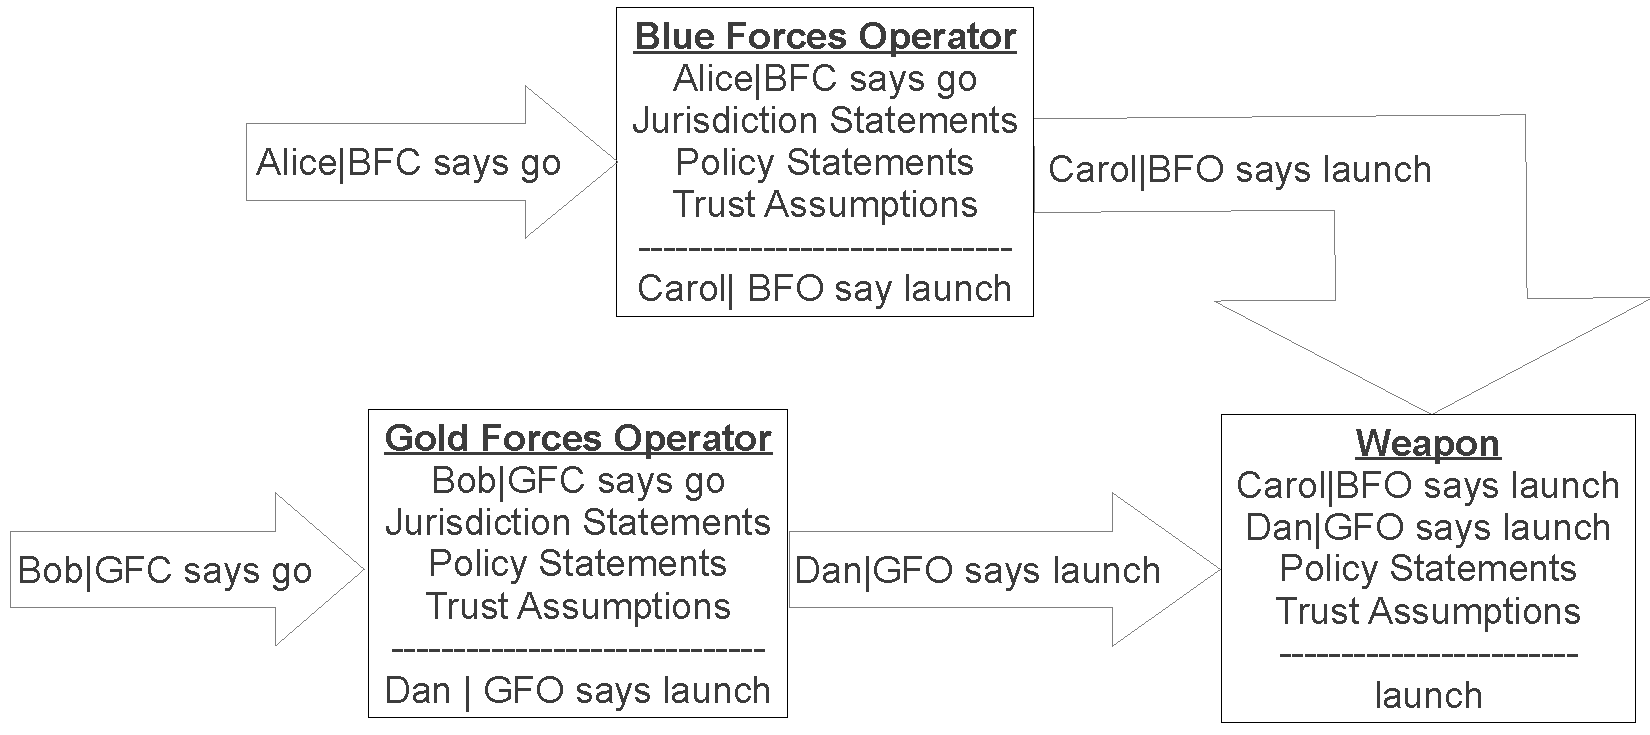
\includegraphics[width=0.95\linewidth]{Figures/launchCONOPSRefine1}}
    \end{minipage}
    &
    \begin{minipage}{0.48\linewidth}
      \centering{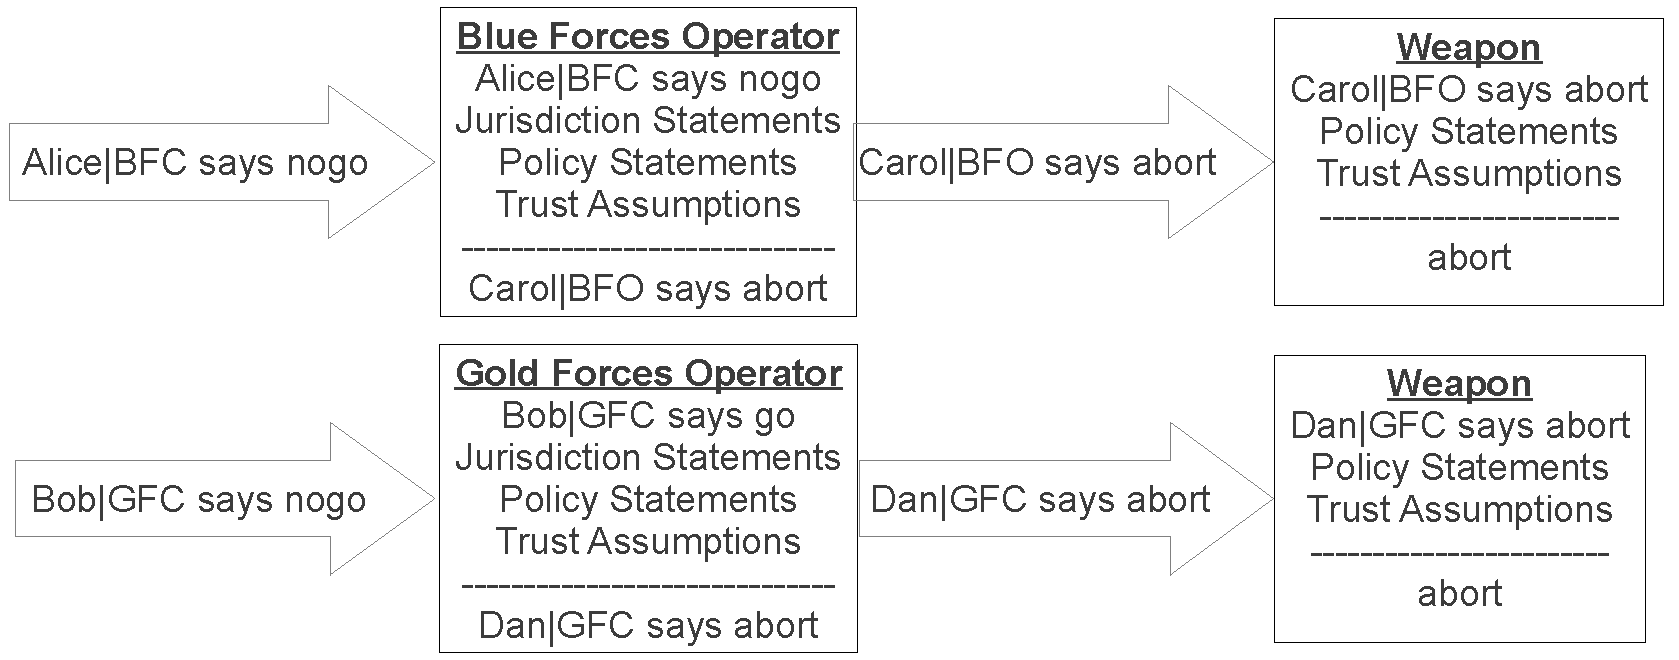
\includegraphics[width=0.95\linewidth]{Figures/abortCONOPSRefine1}}
    \end{minipage}\\
    (a) Launch CONOPS & (b) Abort CONOPS\\
  \end{tabular}
  
  \caption{Launch and Abort CONOPS with Assigned Personnel}
  \label{fig:conops-with-people}
\end{figure}

\begin{table}[t]
  \centering
  \begin{tabular}{|c|c|>{$}l<{$}|}
    \hline
    \textbf{Role} & \textbf{Description of Authority} & 
    \textbf{Formal Description of Authority}\\
    \hline
    Blue Forces Commander (BFC) & go & BFC \controls \action{go}\\
    & nogo & BFC \controls \action{nogo}\\
    & Assignment of BF Operators & BFC \controls (\reps{P}{BFO}{\varphi})\\
    \hline
    Gold Forces Commander (GFC) & go & GFC \controls \action{go}\\
    & nogo & GFC \controls \action{nogo}\\
    & Assignment of GF Operators & GFC \controls (\reps{P}{GFO}{\varphi})\\
    \hline
    Blue Forces Operator (BFO) & launch & BFO \controls \action{launch}\\
    & abort & BFO \controls \action{abort}\\
    \hline
    Gold Forces Operator (GFO) & launch & GFO \controls \action{launch}\\
    & abort & GFO \controls \action{abort}\\
    \hline
  \end{tabular}
  \caption{Mission Roles and Their Authority}
  \label{tab:roles-authority}
\end{table}
\begin{table}[t]
  \centering
  \begin{center}
  \begin{tabular}[h]{|r|l|l|>{$}p{0.43\linewidth}<{$}|}
    \hline
    \textbf{Role} & \textbf{Person} & \textbf{Authenticated By} & \textbf{Formal Description of Delegation of Authority}\\
    \hline
    BFC & Alice & pre-distributed prior to mission & 
    \reps{Alice}{BFC}{\varphi} \\
    & & & \reps{Alice}{BFC}{(\reps{Carol}{BFO}{\varphi})}\\
    GFC & Bob & pre-distributed prior to mission & 
    \reps{Bob}{GFC}{\varphi}\\
    & & & \reps{Bob}{GFC}{(\reps{Dan}{GFO}{\varphi})}\\
    BFO & Carol & Alice as BFC & \reps{Carol}{BFO}{\varphi}\\
    GFO & Dan & Bob as GFC & \reps{Dan}{GFO}{\varphi}\\
    \hline
  \end{tabular}
\end{center}
\caption{Role Assignments and Authorizations}
\label{tab:role-assignments}
\end{table}

The first refinement to the high-level CONOPS expressed only in terms
of mission roles is to add the notion of authentication of principals
acting in mission roles. A principal $P$ acting in a mission role
\emph{Role} giving command $\varphi$ is represented by $P \quoting
Role \says \varphi$. If \emph{P's} authority to act in role
\emph{Role} is recognized, i.e., $\reps{P}{Role}{\varphi}$, and if
$Role \controls \varphi$, then we conclude $\varphi$ is justified,
from the \emph{Reps} inference rule shown below:
\begin{gather*}
  \irule
  {Q \controls \varphi \quad \reps{P}{Q}{\varphi} \quad 
   P \quoting Q \says \varphi}
  {\varphi}
  {Reps}.
\end{gather*}
Figure~\ref{fig:conops-with-people} is a block diagram that refines
the high-level launch and abort CONOPS in
Figure~\ref{fig:launch-abort-conops}.  The primary differences are in
the messages sent among principals. Instead of mission roles speaking,
principals claiming to be acting in mission roles make
statements. Figure~\ref{fig:conops-with-people} shows Alice acting as
Blue Forces Commander, Bob acting as Gold Forces Commander, Carol
acting as Blue Forces Operator, and Dan acting as Gold Forces
Operator.

From the assumptions in Section~\ref{sec:assumptions}, we recall that
Blue and Gold Forces Commanders have the authority to assign personnel
to the roles of Blue and Gold Operators, respectively:
\begin{gather*}
  BFC \controls (\reps{P}{BFO}{\varphi})\\
  GFC \controls (\reps{P}{GFO}{\varphi}).
\end{gather*}
Table~\ref{tab:roles-authority} gives a complete listing of roles and
their associated authority. Table~\ref{tab:role-assignments} shows the
personnel assignments to mission roles and who authenticates them.
Notice that authorizations for personnel designated as Blue and Gold
Forces Commanders are designated as \emph{pre-distributed prior to
  mission}. This is similar to the case where the cryptographic key of
a root certificate authority is pre-loaded into computers. In this
CONOPS, mission equipment and weapons must be loaded with
\textbf{roots of trust} prior to the start of the mission. In this
case, it will include the personnel who are authorized as commanders
as well as cryptographic keys of root authorities. \textbf{The loading
  of this information must be done with the utmost integrity and
  security otherwise all is lost.}

\paragraph{Derived Inference Rules}
\label{sec:deriv-infer-rules}

We now refine the derived inference rules corresponding to BFO Launch,
GFO Launch, BFO Abort, GFO Abort, and when the weapon is launched or
aborted.

\subparagraph{BFO and GFO Launch}
\label{sec:bfo-gfo-launch}

\begin{table}[t]
  \centering
  \begin{tabular}{|r<{.}>{$}l<{$}l|}
    \hline
    1 & Q \controls \varphi_1 & Assumption, jurisdiction of Q\\
    2 & \reps{P}{Q}{\varphi} & P acting in role of Q\\
    3 & P \quoting Q \says \varphi_1 & Command from P\\
    4 & \varphi_1 \implies \varphi_2 & Policy statement\\
    5 & \varphi_1 & 1, 2, 3 Reps\\
    6 & \varphi_2 & 5, 4 Modus Ponens\\
    7 & R \says \varphi_2 & 6 Says\\
    \hline
  \end{tabular}
  \caption{Proof of Implied Controls with Delegation}
  \label{tab:delegation-proof}
\end{table}
Based on Figure~\ref{fig:conops-with-people} we refine the derived
inference rules \emph{BFO Launch} and \emph{GFO Launch} based on the
form of received orders and the trust assumptions and policy
statements needed by operators to issue the launch command to the
weapon.

As we are using delegation of principals to mission roles as a means
for assigning people to mission roles, our launch rules for operators
require operators to know who is operating in the role of Blue or Gold
Forces Commander. This knowledge is reflected in the statements
$\reps{Alice}{BFC}{\action{go}}$ and $\reps{Bob}{GFC}{\action{go}}$.
\begin{gather*}
  \irule
  {
    \begin{array}{c}
      BFC \controls \action{go} \quad \reps{Alice}{BFC}{\action{go}} \quad 
      Alice \quoting BFC \says \action{go} \quad \action{go} \implies \action{launch}
    \end{array}
  }
  {Carol \quoting BFO \says \action{launch}}
  {BFO Launch} \\
  \irule
  {
    \begin{array}{c}
      GFC \controls \action{go} \quad \reps{Bob}{GFC}{\action{go}} \quad 
      Bob \quoting GFC \says \action{go} \quad \action{go} \implies \action{launch}
    \end{array}
  }
  {Dan \quoting GFO \says \action{launch}}
  {GFO Launch}
\end{gather*}
We see that as before both of the Launch rules are instances of the
same rule:
\begin{gather*}
  \irule
  {\begin{array}{c}
      Q \controls \varphi_1 \quad \reps{P}{Q}{\varphi_1} \quad 
      P \quoting Q \says \varphi_1 \quad \varphi_1 \implies \varphi_2
    \end{array}
  }
  {R \says \varphi_2}
  {Implied Controls with Delegation}
\end{gather*}

% \subparagraph{BFO and GFO Abort}
% \label{sec:bfo-gfo-abort}

\begin{center}
  \problembox{
    \begin{enumerate}
    \item Add another LaTeX subparagraph titled \textbf{BFO and GFO
        Abort} that details as \emph{proved inference rules}:
      \begin{enumerate}[{a.}]
      \item when Blue and Gold Forces Operators issue abort commands,
        and
      \item the conditions under which the Weapon will abort.
      \end{enumerate}
    \item Your inference rules should be presented in the style of the
      other inference rules in this section.
    \item Your proofs should be presented in the style of the proofs
      shown in the tables in this section.
    \end{enumerate}

    % A similar set of refinements can be worked out for aborting the
    % mission and the weapon. \textbf{\redtext{Your problem solution
    % will include the refinements for aborting the mission.}}
  }
\end{center}
\subsection{Refined CONOPS Using Cryptographic Keys}
\label{sec:conops-with-keys}

\begin{figure}[t]
  \centering
  \begin{tabular}{cc}
    \begin{minipage}{0.48\linewidth}
      \centering{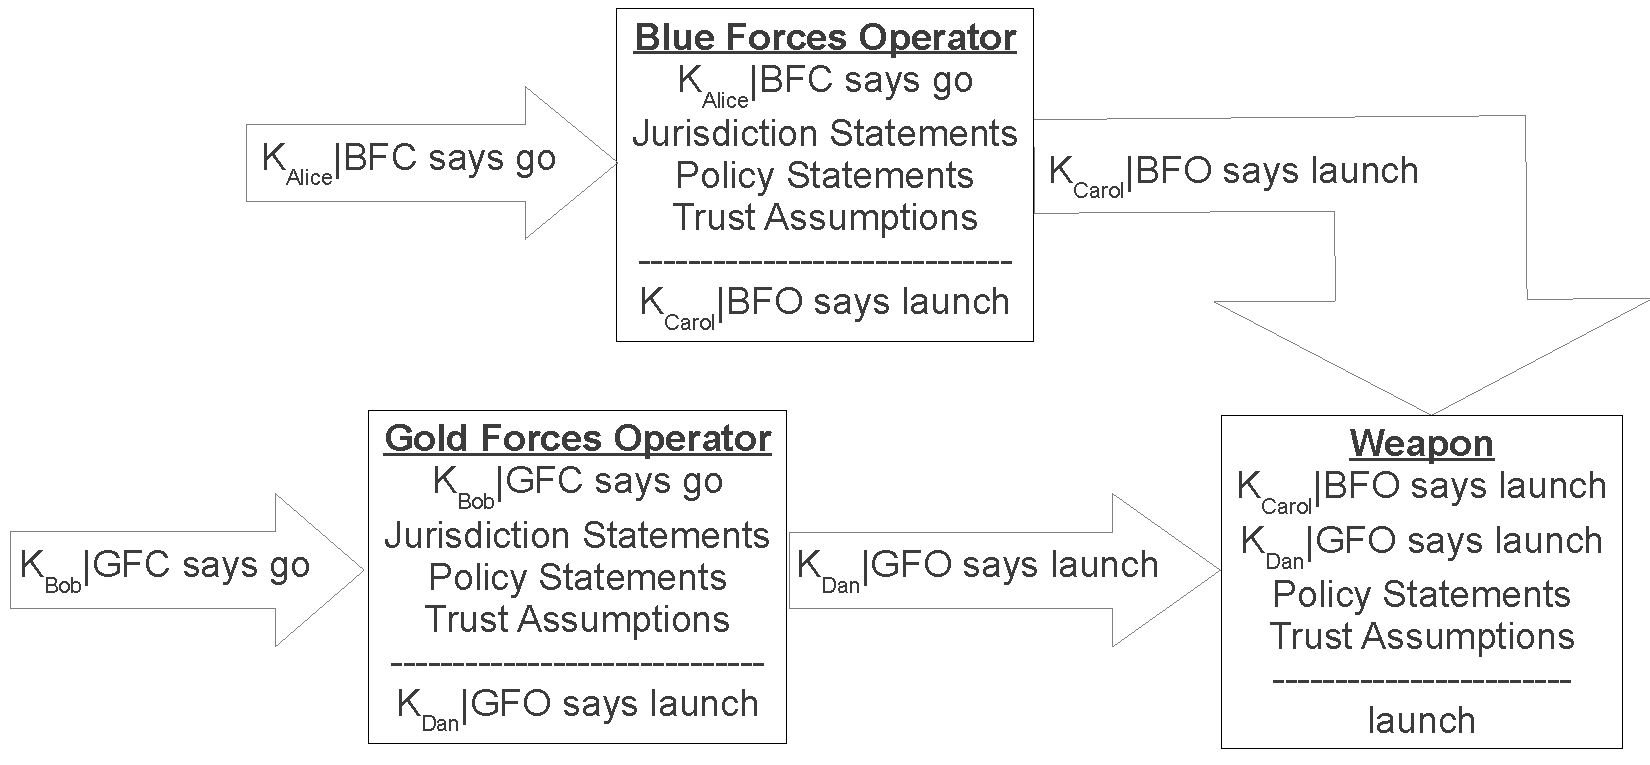
\includegraphics[width=0.95\linewidth]{Figures/launchCONOPSRefine2}}
    \end{minipage}
    &
    \begin{minipage}{0.48\linewidth}
      \centering{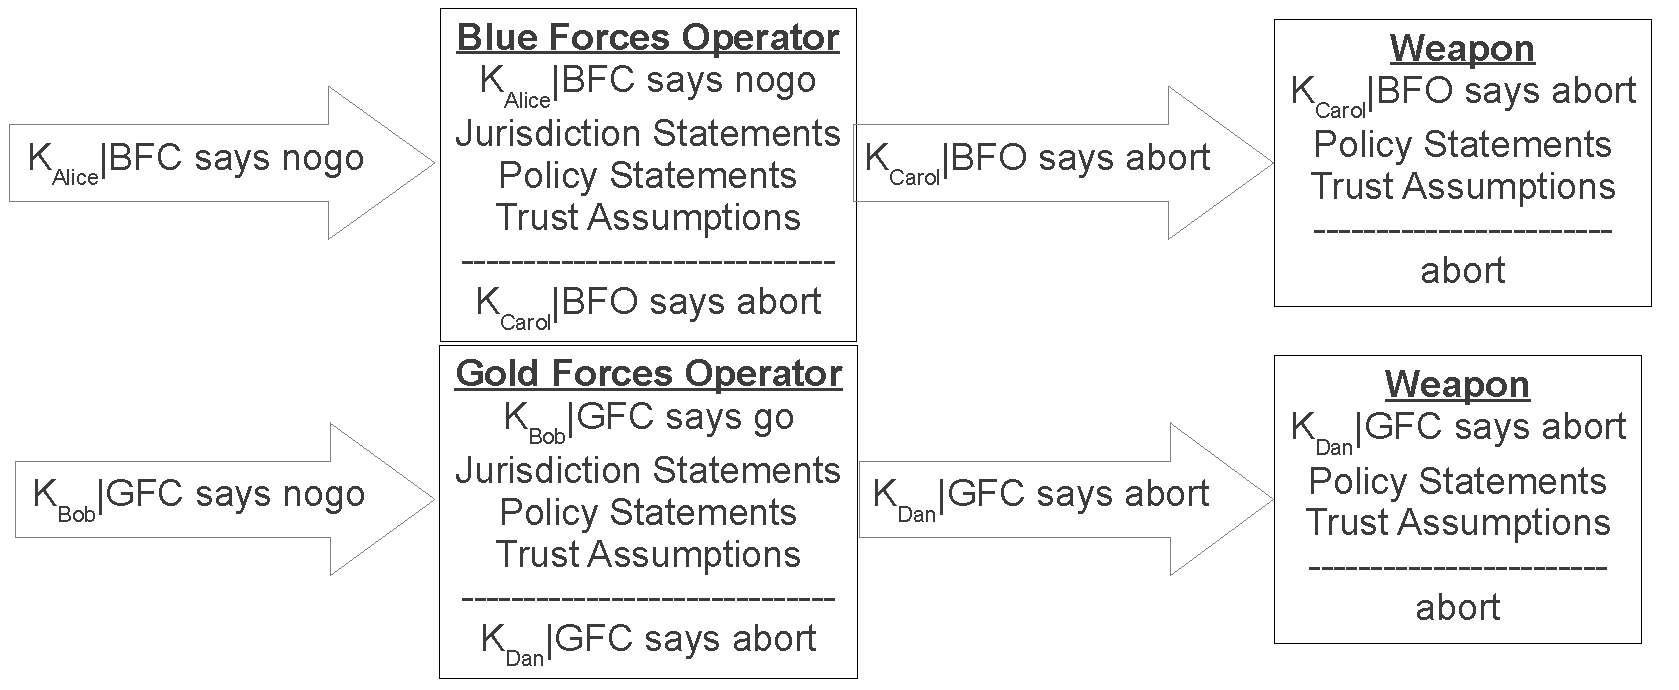
\includegraphics[width=0.95\linewidth]{Figures/abortCONOPSRefine2}}
    \end{minipage}\\
    (a) Launch CONOPS & (b) Abort CONOPS\\
  \end{tabular}
  
  \caption{Launch and Abort CONOPS with Cryptographic Keys}
  \label{fig:launch-abort-conops-crypto}
\end{figure}

\begin{center}
  \problembox{Figure~\ref{fig:launch-abort-conops-crypto} is a CONOPS
    that refines the CONOPS in Figure~\ref{fig:conops-with-people} by
    adding the use of cryptographic keys for identification. Your
    problem solution will:
    \begin{enumerate}
    \item Detail the use of cryptographic keys for authenticating the
      integrity of command and control in this CONOPS.
    \item Your solution
      will work within the certificate hierarchy, flow of command and
      control, and jurisdiction of roles described in the assumptions
      in Section~\ref{sec:assumptions}.
    \item As in the high-level and
      refined CONOPS, your solution will show the logical
      justification for each step in the CONOPS in the form of a
      formally proved derived inference rule.
    \item Your inference rules should be presented in the style of the
      other inference rules in the previous sections.
    \item Your proofs should be presented in the style of the proofs
      shown in the tables in the previous sections.
    \end{enumerate}
}
\end{center}


\section{Formal Description and Verification of CONOPS in HOL}

In this section we give the HOL theories used to describe the CONOPS
at three levels of detail. In Section~\ref{sec:mission-roles-conops}
are the HOL theories used to describe and verify the top-level CONOPS
using only mission roles. Section~\ref{sec:conops-with-assigned-staff}
describes the HOL theories that assign staff to mission
roles. Finally, Section~\ref{sec:conops-with-crypto} shows the
description and verification of how cryptographic keys are added to
the CONOPS.

\subsection{CONOPS Using Only Mission Roles}
\label{sec:mission-roles-conops}

The high-level CONOPS is built on two theories and demonstrated in a
third using custom mission-specific forward inference rules.
\begin{enumerate}
\item \textbf{commandTheory:} defines mission commands and weapon
  commands as datatypes.
\item \textbf{missionRolesTheory:} defines mission roles and proves
  theorems that are the basis for forward inference rules in HOL
  corresponding to derived inference rules in the access-control
  logic.
\item \textbf{ missioninf\_rules.sml:} contains mission-oriented
  forward inference rules.
\item \textbf{missionCONOPS1Theory:} proves theorems corresponding to
  each step in the high-level CONOPS.
\end{enumerate}

\subsubsection{commandTheory}
\label{sec:commandTheory}
In \emph{commandTheory}, we introduce the following datatypes:
\begin{enumerate}
\item \emph{missionCommands}: those commands issued by Blue and Gold
  Forces commanders,
\item \emph{weaponCommands}: those commands issued by Blue and Gold
  Forces operators, and
\item \emph{commands}: a datatype combining both mission and weapons
  commands into a single datatype.  This will be used as our
  underlying datatype for propositions in the HOL implementation of
  our access-control logic definitions and proofs.
\end{enumerate}
The datatypes in commandTheory are:
\HOLcommandDatatypesmissionCommands
\HOLcommandDatatypesweaponCommands
\HOLcommandDatatypescommands

\subsubsection{missionRolesTheory}
\label{sec:missionRolesTheory}

In \emph{missionRolesTheory}, we introduce mission roles as the
missionRoles datatype.
\HOLmissionRolesDatatypesmissionRoles

We also prove the following theorems that are the basis for the
derived inference rules for the high-level CONOPS.

\HOLmissionRolesTheorems

% \paragraph{ImpliedControlsSays\_thm}

% \HOLmissionRolesTheoremsImpliedControlsSaysXXthm

% \paragraph{DualControl\_thm}

% \HOLmissionRolesTheoremsDualControlXXthm

% \paragraph{AlternateControls1\_thm}

% \HOLmissionRolesTheoremsAlternateControlsOneXXthm

% \paragraph{AlternateControls2\_thm}

% \HOLmissionRolesTheoremsAlternateControlsTwoXXthm

\subsubsection{Inference Rules}
\label{sec:inference-rules-1}

\begin{holboxed}
  \begin{Large}
    \texttt{\textbf{ImpliedControlsSays}}\hfill{}\texttt{\textbf{(missioninf\_rules)}}
  \end{Large}
\end{holboxed}

\begin{verbatim}
ImpliedControlsSays : term -> thm -> thm -> thm -> thm
\end{verbatim}

\SYNOPSIS Deduces formula f2 if the principal who says f1, controls
f1, and f1 impf f2.

\DESCRIBE

\begin{scriptsize}
\begin{verbatim}
     A1 |- (M,Oi,Os) sat P says f1  A2 |- (M,Oi,Os) sat P controls f1
                            A3 |- f1 impf f2
     ------------------------------------------------------- ImpliedControlsSays Q
               A1 u A2 u A3 |- (M,Oi,Os) sat Q says f2
\end{verbatim}
\end{scriptsize}


\FAILURE
Fails unless the theorems match in terms of principals and formulas
in the access-control logic.

% \EXAMPLE
% The following application:
% \begin{holboxed}
% \begin{verbatim}
% - val a1 = 
%       ACL_ASSUM 
%       ``(Token:'c Princ) says (Role says f:('a,'c,'d,'e)Form)``;
% \end{verbatim}
% \end{holboxed}
% produces the following result:
% \begin{holboxed}
% \begin{verbatim}
% val a1 =  [.] |- (M,Oi,Os) sat Token says Role says f : thm
% \end{verbatim}
% \end{holboxed}

\IMPLEMENTATION
The implementation is as follows
\begin{holboxed}
\begin{verbatim}
fun ImpliedControlsSays Q th1 th2 th3 =
MATCH_MP (MATCH_MP (MATCH_MP (ISPEC Q ImpliedControlsSays_thm) th1) th2) th3;
\end{verbatim}
\end{holboxed}

\SEEALSO
DualControl, AltControls1, AltControls2, CONTROLS
\ENDDOC

\begin{holboxed}
  \begin{Large}
    \texttt{\textbf{DualControl}}\hfill{}\texttt{\textbf{(missioninf\_rules)}}
  \end{Large}
\end{holboxed}

\begin{verbatim}
DualControl : thm -> thm -> thm -> thm
\end{verbatim}

\SYNOPSIS 
Deduces formula f if P says f, Q says f, and (P meet Q) controls f

\DESCRIBE

\begin{scriptsize}
\begin{verbatim}
 A1 |- (M,Oi,Os) sat P says f  A2 |- (M,Oi,Os) sat Q says f
                     A3 |- (P meet Q) controls f
 ------------------------------------------------------- DualControl
                     A1 u A2 u A3 |- (M,Oi,Os) sat f
\end{verbatim}
\end{scriptsize}


\FAILURE
Fails unless the theorems match in terms of principals and formulas
in the access-control logic.

\IMPLEMENTATION
The implementation is as follows
\begin{holboxed}
\begin{verbatim}
fun DualControl th1 th2 th3 =
MATCH_MP (MATCH_MP (MATCH_MP DualControl_thm th1) th2) th3;
\end{verbatim}
\end{holboxed}

\SEEALSO
ImpliedCOntrolsSays, AltControls1, AltControls2, CONTROLS
\ENDDOC

\begin{holboxed}
  \begin{Large}
    \texttt{\textbf{AltControls1}}\hfill{}\texttt{\textbf{(missioninf\_rules)}}
  \end{Large}
\end{holboxed}

\begin{verbatim}
AltControls1 : thm -> thm -> thm
\end{verbatim}

\SYNOPSIS 
Deduces formula f if P says f and (P controls f andf Q controls f)

\DESCRIBE

\begin{scriptsize}
\begin{verbatim}
  A1 |- (M,Oi,Os) sat P says f A2 |- P controls f andf Q controls f
  ------------------------------------------------------- AltControls1
                      A1 u A2 |- (M,Oi,Os) sat f
\end{verbatim}
\end{scriptsize}

\FAILURE
Fails unless the theorems match in terms of principals and formulas
in the access-control logic.

\IMPLEMENTATION
The implementation is as follows
\begin{holboxed}
\begin{verbatim}
fun AltControls1 th1 th2 =
MATCH_MP (MATCH_MP AlternateControls1_thm th1) th2;
\end{verbatim}
\end{holboxed}

\SEEALSO
ImpliedControlsSays, DualControl, AltControls2, CONTROLS
\ENDDOC

\begin{holboxed}
  \begin{Large}
    \texttt{\textbf{AltControls2}}\hfill{}\texttt{\textbf{(missioninf\_rules)}}
  \end{Large}
\end{holboxed}

\begin{verbatim}
AltControls2 : thm -> thm -> thm
\end{verbatim}

\SYNOPSIS 
Deduces formula f if P says f and (P controls f andf Q controls f)

\DESCRIBE

\begin{scriptsize}
\begin{verbatim}
  A1 |- (M,Oi,Os) sat Q says f A2 |- P controls f andf Q controls f
  ------------------------------------------------------- AltControls2
                      A1 u A2 |- (M,Oi,Os) sat f
\end{verbatim}
\end{scriptsize}

\FAILURE
Fails unless the theorems match in terms of principals and formulas
in the access-control logic.

\IMPLEMENTATION
The implementation is as follows
\begin{holboxed}
\begin{verbatim}
fun AltControls2 th1 th2 =
MATCH_MP (MATCH_MP AlternateControls2_thm th1) th2;
\end{verbatim}
\end{holboxed}

\SEEALSO
ImpliedControlsSays, DualControl, AltControls1, CONTROLS
\ENDDOC
\subsubsection{missionCONOPS1Theory}
\label{sec:missionCONOPS1Theory}

The following theorems are proved in \emph{missionCONOPS1Theory},
which fully accounts for each step in each situation for the
high-level CONOPS.

\HOLmissionCONOPSOneTheorems
\subsection{CONOPS with Staff Assigned to Mission Roles}
\label{sec:conops-with-assigned-staff}

The CONOPS with mission staff assigned to mission roles is built using
\emph{missionStaffTheory} and additional inference rules.
\begin{enumerate}
\item \textbf{missionStaffTheory:} defines mission staff and
  missionRoleStaff that combines both mission roles and staff into a
  single datatype that is the underlying source of principals.
\item \textbf{missioninf\_rules.sml:} contains mission-oriented
  forward inference rules.
\item \textbf{missionCONOPS2Theory:} proves theorems corresponding to
  each step in the staff-level CONOPS.
\end{enumerate}

\subsubsection{missionStaffTheory}
\label{sec:missionStaffTheory}

The \emph{missionStaffTheory} depends on \emph{missionRolesTheory} and
introduces Alice, Bob, Carol, and Dan as mission staff. The theory
introduces \emph{missionRoleStaff} as a datatype as the source of
principals.
\HOLmissionStaffDatatypes

The following theorems are proved that are the basis for the derived
inference rules for the staff-level CONOPS.
\HOLmissionStaffTheorems

\begin{center}
  \problembox{Add whatever additional theorems are necessary for the
    CONOPS.}
\end{center}


\subsubsection{Inference Rules}
\label{sec:inference-rules-2}

\begin{holboxed}
  \begin{Large}
    \texttt{\textbf{ImpliedControlsDelegation}}\hfill{}\texttt{\textbf{(missioninf\_rules)}}
  \end{Large}
\end{holboxed}

\begin{verbatim}
ImpliedControlsDelegation : term -> thm -> thm -> thm -> thm -> thm
\end{verbatim}

\SYNOPSIS 
Deduces formula f2 if a principal quoting a second principal
says f1, where the second principal controls f1, and f1 impf f2.

\DESCRIBE

\begin{scriptsize}
\begin{verbatim}
 A1 |- (M,Oi,Os) sat Q controls f1  A2 |- (M,Oi,Os) sat reps P Q f1
        A3 |- P quoting Q says f1  A4 |- f1 impf f2
 ------------------------------------------------------- ImpliedControlsDelegation R
      A1 u A2 u A3 u A4 |- (M,Oi,Os) sat R says f2
\end{verbatim}
\end{scriptsize}


\FAILURE
Fails unless the theorems match in terms of principals and formulas
in the access-control logic.

\IMPLEMENTATION
The implementation is as follows
\begin{holboxed}
\begin{verbatim}
fun ImpliedControlsDelegation R th1 th2 th3 th4 =
MATCH_MP
(MATCH_MP 
 (MATCH_MP 
  (MATCH_MP (ISPEC R ImpliedControlsDelegation_thm) th1) th2) th3) th4;
\end{verbatim}
\end{holboxed}

\SEEALSO
ImpliedControlsSays, AltControls1, AltControls1, AltControls2, CONTROLS
\ENDDOC

\begin{center}
  \problembox{Add whatever mission-oriented inference rules are
    necessary for the staff-oriented CONOPS.}
\end{center}
\subsubsection{missionCONOPS2Theory}
\label{sec:missionCONOPS2Theory}

The following theorems are proved for each step of the staff-oriented CONOPS.

\HOLmissionCONOPSTwoTheorems

\begin{center}
  \problembox{Prove and add the theorems corresponding to the
    remaining steps in the staff-oriented CONOPS for operator aborts,
    weapon launch, and weapon abort.}
\end{center}

\subsection{CONOPS with Cryptographic Keys}
\label{sec:conops-with-crypto}

The CONOPS with cryptographic keys assigned to staff in mission roles is built using
\emph{missionKeysTheory} and additional inference rules.
\begin{enumerate}
\item \textbf{missionKeysTheory:} defines mission certificate
  authorities, keys, staff, roles, and mission principals that
  combines both mission keys, staff, and roles into a single datatype
  that is the underlying source of mission principals.
\item \textbf{missioninf\_rules.sml:} contains mission-oriented
  forward inference rules.
\item \textbf{missionCONOPS3Theory:} proves theorems corresponding to
  each step in the crypto-level CONOPS.
\end{enumerate}

\subsubsection{missionKeysTheory}
\label{sec:missionKeysTheory}

\HOLmissionKeysDatatypes

\begin{center}
  \problembox{Add the necessary theorems needed for your inference
    rules to justify each step in the crypto-level CONOPS.}
\end{center}

\subsubsection{Inference Rules}
\label{sec:inference-rules-3}

\begin{center}
  \problembox{Add the necessary inference needed rules to justify each
    step in the crypto-level CONOPS.}
\end{center}

\subsubsection{missionCONOPS3Theory}
\label{sec:missionCONOPS3Theory}

\begin{center}
  \problembox{Develop this theory to demonstrate the validity of your
    CONOPS at the crypto level.}
\end{center}
\section{Risk Assessment}

\begin{center}
  \problembox{
    \begin{enumerate}
    \item Add your assessment of risks for the CONOPS.
    \item Comment on the importance and means by which the
      pre-distribution of root keys and authorities is done and the
      risks involved.
    \end{enumerate}
}
\end{center}


\bibliography{references}
\bibliographystyle{alpha}

\newpage{}
\part*{Appendices}
\label{part:appendices}

\begin{center}
  \problembox{Update the files and theories with your solutions and
    source code.}
\end{center}

\documentclass[11pt, twoside]{article}
\usepackage{holtex}

\makeindex

\begin{document}

\newcommand{\HOLcommandDate}{20 August 2016}
\newcommand{\HOLcommandTime}{11:38}
\begin{SaveVerbatim}{HOLcommandDatatypescommands}
\HOLFreeVar{commands} = \HOLConst{MC} \HOLTyOp{missionCommands} \HOLTokenBar{} \HOLConst{WC} \HOLTyOp{weaponCommands}
\end{SaveVerbatim}
\newcommand{\HOLcommandDatatypescommands}{\UseVerbatim{HOLcommandDatatypescommands}}
\begin{SaveVerbatim}{HOLcommandDatatypesmissionCommands}
\HOLFreeVar{missionCommands} = \HOLConst{go} \HOLTokenBar{} \HOLConst{nogo}
\end{SaveVerbatim}
\newcommand{\HOLcommandDatatypesmissionCommands}{\UseVerbatim{HOLcommandDatatypesmissionCommands}}
\begin{SaveVerbatim}{HOLcommandDatatypesweaponCommands}
\HOLFreeVar{weaponCommands} = \HOLConst{launch} \HOLTokenBar{} \HOLConst{abort}
\end{SaveVerbatim}
\newcommand{\HOLcommandDatatypesweaponCommands}{\UseVerbatim{HOLcommandDatatypesweaponCommands}}
\newcommand{\HOLcommandDatatypes}{
\HOLcommandDatatypescommands\HOLcommandDatatypesmissionCommands\HOLcommandDatatypesweaponCommands}

\newcommand{\HOLmissionRolesDate}{20 August 2016}
\newcommand{\HOLmissionRolesTime}{11:38}
\begin{SaveVerbatim}{HOLmissionRolesDatatypesmissionRoles}
\HOLFreeVar{missionRoles} = \HOLConst{BFC} \HOLTokenBar{} \HOLConst{GFC} \HOLTokenBar{} \HOLConst{BFO} \HOLTokenBar{} \HOLConst{GFO}
\end{SaveVerbatim}
\newcommand{\HOLmissionRolesDatatypesmissionRoles}{\UseVerbatim{HOLmissionRolesDatatypesmissionRoles}}
\newcommand{\HOLmissionRolesDatatypes}{
\HOLmissionRolesDatatypesmissionRoles}
\begin{SaveVerbatim}{HOLmissionRolesTheoremsAlternateControlsOneXXthm}
\HOLTokenTurnstile{} (\HOLFreeVar{M}\HOLSymConst{,}\HOLFreeVar{Oi}\HOLSymConst{,}\HOLFreeVar{Os}) \HOLConst{sat} \HOLFreeVar{P} \HOLConst{says} \HOLFreeVar{f} \HOLSymConst{\HOLTokenImp{}}
   (\HOLFreeVar{M}\HOLSymConst{,}\HOLFreeVar{Oi}\HOLSymConst{,}\HOLFreeVar{Os}) \HOLConst{sat} \HOLFreeVar{P} \HOLConst{controls} \HOLFreeVar{f} \HOLConst{andf} \HOLFreeVar{Q} \HOLConst{controls} \HOLFreeVar{f} \HOLSymConst{\HOLTokenImp{}}
   (\HOLFreeVar{M}\HOLSymConst{,}\HOLFreeVar{Oi}\HOLSymConst{,}\HOLFreeVar{Os}) \HOLConst{sat} \HOLFreeVar{f}
\end{SaveVerbatim}
\newcommand{\HOLmissionRolesTheoremsAlternateControlsOneXXthm}{\UseVerbatim{HOLmissionRolesTheoremsAlternateControlsOneXXthm}}
\begin{SaveVerbatim}{HOLmissionRolesTheoremsAlternateControlsTwoXXthm}
\HOLTokenTurnstile{} (\HOLFreeVar{M}\HOLSymConst{,}\HOLFreeVar{Oi}\HOLSymConst{,}\HOLFreeVar{Os}) \HOLConst{sat} \HOLFreeVar{Q} \HOLConst{says} \HOLFreeVar{f} \HOLSymConst{\HOLTokenImp{}}
   (\HOLFreeVar{M}\HOLSymConst{,}\HOLFreeVar{Oi}\HOLSymConst{,}\HOLFreeVar{Os}) \HOLConst{sat} \HOLFreeVar{P} \HOLConst{controls} \HOLFreeVar{f} \HOLConst{andf} \HOLFreeVar{Q} \HOLConst{controls} \HOLFreeVar{f} \HOLSymConst{\HOLTokenImp{}}
   (\HOLFreeVar{M}\HOLSymConst{,}\HOLFreeVar{Oi}\HOLSymConst{,}\HOLFreeVar{Os}) \HOLConst{sat} \HOLFreeVar{f}
\end{SaveVerbatim}
\newcommand{\HOLmissionRolesTheoremsAlternateControlsTwoXXthm}{\UseVerbatim{HOLmissionRolesTheoremsAlternateControlsTwoXXthm}}
\begin{SaveVerbatim}{HOLmissionRolesTheoremsDualControlXXthm}
\HOLTokenTurnstile{} (\HOLFreeVar{M}\HOLSymConst{,}\HOLFreeVar{Oi}\HOLSymConst{,}\HOLFreeVar{Os}) \HOLConst{sat} \HOLFreeVar{P} \HOLConst{says} \HOLFreeVar{s} \HOLSymConst{\HOLTokenImp{}}
   (\HOLFreeVar{M}\HOLSymConst{,}\HOLFreeVar{Oi}\HOLSymConst{,}\HOLFreeVar{Os}) \HOLConst{sat} \HOLFreeVar{Q} \HOLConst{says} \HOLFreeVar{s} \HOLSymConst{\HOLTokenImp{}}
   (\HOLFreeVar{M}\HOLSymConst{,}\HOLFreeVar{Oi}\HOLSymConst{,}\HOLFreeVar{Os}) \HOLConst{sat} \HOLFreeVar{P} \HOLConst{meet} \HOLFreeVar{Q} \HOLConst{controls} \HOLFreeVar{s} \HOLSymConst{\HOLTokenImp{}}
   (\HOLFreeVar{M}\HOLSymConst{,}\HOLFreeVar{Oi}\HOLSymConst{,}\HOLFreeVar{Os}) \HOLConst{sat} \HOLFreeVar{s}
\end{SaveVerbatim}
\newcommand{\HOLmissionRolesTheoremsDualControlXXthm}{\UseVerbatim{HOLmissionRolesTheoremsDualControlXXthm}}
\begin{SaveVerbatim}{HOLmissionRolesTheoremsImpliedControlsSaysXXthm}
\HOLTokenTurnstile{} \HOLSymConst{\HOLTokenForall{}}\HOLBoundVar{Q}.
     (\HOLFreeVar{M}\HOLSymConst{,}\HOLFreeVar{Oi}\HOLSymConst{,}\HOLFreeVar{Os}) \HOLConst{sat} \HOLFreeVar{P} \HOLConst{says} \HOLFreeVar{s\sb{\mathrm{1}}} \HOLSymConst{\HOLTokenImp{}}
     (\HOLFreeVar{M}\HOLSymConst{,}\HOLFreeVar{Oi}\HOLSymConst{,}\HOLFreeVar{Os}) \HOLConst{sat} \HOLFreeVar{P} \HOLConst{controls} \HOLFreeVar{s\sb{\mathrm{1}}} \HOLSymConst{\HOLTokenImp{}}
     (\HOLFreeVar{M}\HOLSymConst{,}\HOLFreeVar{Oi}\HOLSymConst{,}\HOLFreeVar{Os}) \HOLConst{sat} \HOLFreeVar{s\sb{\mathrm{1}}} \HOLConst{impf} \HOLFreeVar{s\sb{\mathrm{2}}} \HOLSymConst{\HOLTokenImp{}}
     (\HOLFreeVar{M}\HOLSymConst{,}\HOLFreeVar{Oi}\HOLSymConst{,}\HOLFreeVar{Os}) \HOLConst{sat} \HOLBoundVar{Q} \HOLConst{says} \HOLFreeVar{s\sb{\mathrm{2}}}
\end{SaveVerbatim}
\newcommand{\HOLmissionRolesTheoremsImpliedControlsSaysXXthm}{\UseVerbatim{HOLmissionRolesTheoremsImpliedControlsSaysXXthm}}
\newcommand{\HOLmissionRolesTheorems}{
\HOLThmTag{missionRoles}{AlternateControls1_thm}\HOLmissionRolesTheoremsAlternateControlsOneXXthm
\HOLThmTag{missionRoles}{AlternateControls2_thm}\HOLmissionRolesTheoremsAlternateControlsTwoXXthm
\HOLThmTag{missionRoles}{DualControl_thm}\HOLmissionRolesTheoremsDualControlXXthm
\HOLThmTag{missionRoles}{ImpliedControlsSays_thm}\HOLmissionRolesTheoremsImpliedControlsSaysXXthm
}

\newcommand{\HOLmissionCONOPSOneDate}{20 August 2016}
\newcommand{\HOLmissionCONOPSOneTime}{11:38}
\begin{SaveVerbatim}{HOLmissionCONOPSOneTheoremsBFOXXabortXXthm}
\HOLTokenTurnstile{} (\HOLFreeVar{M}\HOLSymConst{,}\HOLFreeVar{Oi}\HOLSymConst{,}\HOLFreeVar{Os}) \HOLConst{sat} \HOLConst{Name} \HOLConst{BFC} \HOLConst{says} \HOLConst{prop} (\HOLConst{MC} \HOLConst{nogo}) \HOLSymConst{\HOLTokenImp{}}
   (\HOLFreeVar{M}\HOLSymConst{,}\HOLFreeVar{Oi}\HOLSymConst{,}\HOLFreeVar{Os}) \HOLConst{sat} \HOLConst{prop} (\HOLConst{MC} \HOLConst{nogo}) \HOLConst{impf} \HOLConst{prop} (\HOLConst{WC} \HOLConst{abort}) \HOLSymConst{\HOLTokenImp{}}
   (\HOLFreeVar{M}\HOLSymConst{,}\HOLFreeVar{Oi}\HOLSymConst{,}\HOLFreeVar{Os}) \HOLConst{sat} \HOLConst{Name} \HOLConst{BFC} \HOLConst{controls} \HOLConst{prop} (\HOLConst{MC} \HOLConst{nogo}) \HOLSymConst{\HOLTokenImp{}}
   (\HOLFreeVar{M}\HOLSymConst{,}\HOLFreeVar{Oi}\HOLSymConst{,}\HOLFreeVar{Os}) \HOLConst{sat} \HOLConst{Name} \HOLConst{BFO} \HOLConst{says} \HOLConst{prop} (\HOLConst{WC} \HOLConst{abort})
\end{SaveVerbatim}
\newcommand{\HOLmissionCONOPSOneTheoremsBFOXXabortXXthm}{\UseVerbatim{HOLmissionCONOPSOneTheoremsBFOXXabortXXthm}}
\begin{SaveVerbatim}{HOLmissionCONOPSOneTheoremsBFOXXlaunchXXthm}
\HOLTokenTurnstile{} (\HOLFreeVar{M}\HOLSymConst{,}\HOLFreeVar{Oi}\HOLSymConst{,}\HOLFreeVar{Os}) \HOLConst{sat} \HOLConst{Name} \HOLConst{BFC} \HOLConst{says} \HOLConst{prop} (\HOLConst{MC} \HOLConst{go}) \HOLSymConst{\HOLTokenImp{}}
   (\HOLFreeVar{M}\HOLSymConst{,}\HOLFreeVar{Oi}\HOLSymConst{,}\HOLFreeVar{Os}) \HOLConst{sat} \HOLConst{prop} (\HOLConst{MC} \HOLConst{go}) \HOLConst{impf} \HOLConst{prop} (\HOLConst{WC} \HOLConst{launch}) \HOLSymConst{\HOLTokenImp{}}
   (\HOLFreeVar{M}\HOLSymConst{,}\HOLFreeVar{Oi}\HOLSymConst{,}\HOLFreeVar{Os}) \HOLConst{sat} \HOLConst{Name} \HOLConst{BFC} \HOLConst{controls} \HOLConst{prop} (\HOLConst{MC} \HOLConst{go}) \HOLSymConst{\HOLTokenImp{}}
   (\HOLFreeVar{M}\HOLSymConst{,}\HOLFreeVar{Oi}\HOLSymConst{,}\HOLFreeVar{Os}) \HOLConst{sat} \HOLConst{Name} \HOLConst{BFO} \HOLConst{says} \HOLConst{prop} (\HOLConst{WC} \HOLConst{launch})
\end{SaveVerbatim}
\newcommand{\HOLmissionCONOPSOneTheoremsBFOXXlaunchXXthm}{\UseVerbatim{HOLmissionCONOPSOneTheoremsBFOXXlaunchXXthm}}
\begin{SaveVerbatim}{HOLmissionCONOPSOneTheoremsBFOXXweaponsXXabortXXthm}
\HOLTokenTurnstile{} (\HOLFreeVar{M}\HOLSymConst{,}\HOLFreeVar{Oi}\HOLSymConst{,}\HOLFreeVar{Os}) \HOLConst{sat} \HOLConst{Name} \HOLConst{BFO} \HOLConst{says} \HOLConst{prop} (\HOLConst{WC} \HOLConst{abort}) \HOLSymConst{\HOLTokenImp{}}
   (\HOLFreeVar{M}\HOLSymConst{,}\HOLFreeVar{Oi}\HOLSymConst{,}\HOLFreeVar{Os}) \HOLConst{sat}
   \HOLConst{Name} \HOLConst{BFO} \HOLConst{controls} \HOLConst{prop} (\HOLConst{WC} \HOLConst{abort}) \HOLConst{andf}
   \HOLConst{Name} \HOLConst{GFO} \HOLConst{controls} \HOLConst{prop} (\HOLConst{WC} \HOLConst{abort}) \HOLSymConst{\HOLTokenImp{}}
   (\HOLFreeVar{M}\HOLSymConst{,}\HOLFreeVar{Oi}\HOLSymConst{,}\HOLFreeVar{Os}) \HOLConst{sat} \HOLConst{prop} (\HOLConst{WC} \HOLConst{abort})
\end{SaveVerbatim}
\newcommand{\HOLmissionCONOPSOneTheoremsBFOXXweaponsXXabortXXthm}{\UseVerbatim{HOLmissionCONOPSOneTheoremsBFOXXweaponsXXabortXXthm}}
\begin{SaveVerbatim}{HOLmissionCONOPSOneTheoremsGFOXXabortXXthm}
\HOLTokenTurnstile{} (\HOLFreeVar{M}\HOLSymConst{,}\HOLFreeVar{Oi}\HOLSymConst{,}\HOLFreeVar{Os}) \HOLConst{sat} \HOLConst{Name} \HOLConst{GFC} \HOLConst{says} \HOLConst{prop} (\HOLConst{MC} \HOLConst{nogo}) \HOLSymConst{\HOLTokenImp{}}
   (\HOLFreeVar{M}\HOLSymConst{,}\HOLFreeVar{Oi}\HOLSymConst{,}\HOLFreeVar{Os}) \HOLConst{sat} \HOLConst{prop} (\HOLConst{MC} \HOLConst{nogo}) \HOLConst{impf} \HOLConst{prop} (\HOLConst{WC} \HOLConst{abort}) \HOLSymConst{\HOLTokenImp{}}
   (\HOLFreeVar{M}\HOLSymConst{,}\HOLFreeVar{Oi}\HOLSymConst{,}\HOLFreeVar{Os}) \HOLConst{sat} \HOLConst{Name} \HOLConst{GFC} \HOLConst{controls} \HOLConst{prop} (\HOLConst{MC} \HOLConst{nogo}) \HOLSymConst{\HOLTokenImp{}}
   (\HOLFreeVar{M}\HOLSymConst{,}\HOLFreeVar{Oi}\HOLSymConst{,}\HOLFreeVar{Os}) \HOLConst{sat} \HOLConst{Name} \HOLConst{GFO} \HOLConst{says} \HOLConst{prop} (\HOLConst{WC} \HOLConst{abort})
\end{SaveVerbatim}
\newcommand{\HOLmissionCONOPSOneTheoremsGFOXXabortXXthm}{\UseVerbatim{HOLmissionCONOPSOneTheoremsGFOXXabortXXthm}}
\begin{SaveVerbatim}{HOLmissionCONOPSOneTheoremsGFOXXlaunchXXthm}
\HOLTokenTurnstile{} (\HOLFreeVar{M}\HOLSymConst{,}\HOLFreeVar{Oi}\HOLSymConst{,}\HOLFreeVar{Os}) \HOLConst{sat} \HOLConst{Name} \HOLConst{GFC} \HOLConst{says} \HOLConst{prop} (\HOLConst{MC} \HOLConst{go}) \HOLSymConst{\HOLTokenImp{}}
   (\HOLFreeVar{M}\HOLSymConst{,}\HOLFreeVar{Oi}\HOLSymConst{,}\HOLFreeVar{Os}) \HOLConst{sat} \HOLConst{prop} (\HOLConst{MC} \HOLConst{go}) \HOLConst{impf} \HOLConst{prop} (\HOLConst{WC} \HOLConst{launch}) \HOLSymConst{\HOLTokenImp{}}
   (\HOLFreeVar{M}\HOLSymConst{,}\HOLFreeVar{Oi}\HOLSymConst{,}\HOLFreeVar{Os}) \HOLConst{sat} \HOLConst{Name} \HOLConst{GFC} \HOLConst{controls} \HOLConst{prop} (\HOLConst{MC} \HOLConst{go}) \HOLSymConst{\HOLTokenImp{}}
   (\HOLFreeVar{M}\HOLSymConst{,}\HOLFreeVar{Oi}\HOLSymConst{,}\HOLFreeVar{Os}) \HOLConst{sat} \HOLConst{Name} \HOLConst{GFO} \HOLConst{says} \HOLConst{prop} (\HOLConst{WC} \HOLConst{launch})
\end{SaveVerbatim}
\newcommand{\HOLmissionCONOPSOneTheoremsGFOXXlaunchXXthm}{\UseVerbatim{HOLmissionCONOPSOneTheoremsGFOXXlaunchXXthm}}
\begin{SaveVerbatim}{HOLmissionCONOPSOneTheoremsGFOXXweaponsXXabortXXthm}
\HOLTokenTurnstile{} (\HOLFreeVar{M}\HOLSymConst{,}\HOLFreeVar{Oi}\HOLSymConst{,}\HOLFreeVar{Os}) \HOLConst{sat} \HOLConst{Name} \HOLConst{GFO} \HOLConst{says} \HOLConst{prop} (\HOLConst{WC} \HOLConst{abort}) \HOLSymConst{\HOLTokenImp{}}
   (\HOLFreeVar{M}\HOLSymConst{,}\HOLFreeVar{Oi}\HOLSymConst{,}\HOLFreeVar{Os}) \HOLConst{sat}
   \HOLConst{Name} \HOLConst{BFO} \HOLConst{controls} \HOLConst{prop} (\HOLConst{WC} \HOLConst{abort}) \HOLConst{andf}
   \HOLConst{Name} \HOLConst{GFO} \HOLConst{controls} \HOLConst{prop} (\HOLConst{WC} \HOLConst{abort}) \HOLSymConst{\HOLTokenImp{}}
   (\HOLFreeVar{M}\HOLSymConst{,}\HOLFreeVar{Oi}\HOLSymConst{,}\HOLFreeVar{Os}) \HOLConst{sat} \HOLConst{prop} (\HOLConst{WC} \HOLConst{abort})
\end{SaveVerbatim}
\newcommand{\HOLmissionCONOPSOneTheoremsGFOXXweaponsXXabortXXthm}{\UseVerbatim{HOLmissionCONOPSOneTheoremsGFOXXweaponsXXabortXXthm}}
\begin{SaveVerbatim}{HOLmissionCONOPSOneTheoremsWeaponsXXlaunchXXthm}
\HOLTokenTurnstile{} (\HOLFreeVar{M}\HOLSymConst{,}\HOLFreeVar{Oi}\HOLSymConst{,}\HOLFreeVar{Os}) \HOLConst{sat} \HOLConst{Name} \HOLConst{GFO} \HOLConst{says} \HOLConst{prop} (\HOLConst{WC} \HOLConst{launch}) \HOLSymConst{\HOLTokenImp{}}
   (\HOLFreeVar{M}\HOLSymConst{,}\HOLFreeVar{Oi}\HOLSymConst{,}\HOLFreeVar{Os}) \HOLConst{sat} \HOLConst{Name} \HOLConst{BFO} \HOLConst{says} \HOLConst{prop} (\HOLConst{WC} \HOLConst{launch}) \HOLSymConst{\HOLTokenImp{}}
   (\HOLFreeVar{M}\HOLSymConst{,}\HOLFreeVar{Oi}\HOLSymConst{,}\HOLFreeVar{Os}) \HOLConst{sat}
   \HOLConst{Name} \HOLConst{BFO} \HOLConst{meet} \HOLConst{Name} \HOLConst{GFO} \HOLConst{controls} \HOLConst{prop} (\HOLConst{WC} \HOLConst{launch}) \HOLSymConst{\HOLTokenImp{}}
   (\HOLFreeVar{M}\HOLSymConst{,}\HOLFreeVar{Oi}\HOLSymConst{,}\HOLFreeVar{Os}) \HOLConst{sat} \HOLConst{prop} (\HOLConst{WC} \HOLConst{launch})
\end{SaveVerbatim}
\newcommand{\HOLmissionCONOPSOneTheoremsWeaponsXXlaunchXXthm}{\UseVerbatim{HOLmissionCONOPSOneTheoremsWeaponsXXlaunchXXthm}}
\newcommand{\HOLmissionCONOPSOneTheorems}{
\HOLThmTag{missionCONOPS1}{BFO_abort_thm}\HOLmissionCONOPSOneTheoremsBFOXXabortXXthm
\HOLThmTag{missionCONOPS1}{BFO_launch_thm}\HOLmissionCONOPSOneTheoremsBFOXXlaunchXXthm
\HOLThmTag{missionCONOPS1}{BFO_weapons_abort_thm}\HOLmissionCONOPSOneTheoremsBFOXXweaponsXXabortXXthm
\HOLThmTag{missionCONOPS1}{GFO_abort_thm}\HOLmissionCONOPSOneTheoremsGFOXXabortXXthm
\HOLThmTag{missionCONOPS1}{GFO_launch_thm}\HOLmissionCONOPSOneTheoremsGFOXXlaunchXXthm
\HOLThmTag{missionCONOPS1}{GFO_weapons_abort_thm}\HOLmissionCONOPSOneTheoremsGFOXXweaponsXXabortXXthm
\HOLThmTag{missionCONOPS1}{Weapons_launch_thm}\HOLmissionCONOPSOneTheoremsWeaponsXXlaunchXXthm
}

\newcommand{\HOLmissionStaffDate}{20 August 2016}
\newcommand{\HOLmissionStaffTime}{11:38}
\begin{SaveVerbatim}{HOLmissionStaffDatatypesmissionRoleStaff}
\HOLFreeVar{missionRoleStaff} = \HOLConst{Role} \HOLTyOp{missionRoles} \HOLTokenBar{} \HOLConst{Staff} \HOLTyOp{missionStaff}
\end{SaveVerbatim}
\newcommand{\HOLmissionStaffDatatypesmissionRoleStaff}{\UseVerbatim{HOLmissionStaffDatatypesmissionRoleStaff}}
\begin{SaveVerbatim}{HOLmissionStaffDatatypesmissionStaff}
\HOLFreeVar{missionStaff} = \HOLConst{Alice} \HOLTokenBar{} \HOLConst{Bob} \HOLTokenBar{} \HOLConst{Carol} \HOLTokenBar{} \HOLConst{Dan} \HOLTokenBar{} \HOLConst{Weapon}
\end{SaveVerbatim}
\newcommand{\HOLmissionStaffDatatypesmissionStaff}{\UseVerbatim{HOLmissionStaffDatatypesmissionStaff}}
\newcommand{\HOLmissionStaffDatatypes}{
\HOLmissionStaffDatatypesmissionRoleStaff\HOLmissionStaffDatatypesmissionStaff}
\begin{SaveVerbatim}{HOLmissionStaffTheoremsImpliedControlsDelegationXXthm}
\HOLTokenTurnstile{} \HOLSymConst{\HOLTokenForall{}}\HOLBoundVar{R}.
     (\HOLFreeVar{M}\HOLSymConst{,}\HOLFreeVar{Oi}\HOLSymConst{,}\HOLFreeVar{Os}) \HOLConst{sat} \HOLFreeVar{Q} \HOLConst{controls} \HOLFreeVar{f\sb{\mathrm{1}}} \HOLSymConst{\HOLTokenImp{}}
     (\HOLFreeVar{M}\HOLSymConst{,}\HOLFreeVar{Oi}\HOLSymConst{,}\HOLFreeVar{Os}) \HOLConst{sat} \HOLConst{reps} \HOLFreeVar{P} \HOLFreeVar{Q} \HOLFreeVar{f\sb{\mathrm{1}}} \HOLSymConst{\HOLTokenImp{}}
     (\HOLFreeVar{M}\HOLSymConst{,}\HOLFreeVar{Oi}\HOLSymConst{,}\HOLFreeVar{Os}) \HOLConst{sat} \HOLFreeVar{P} \HOLConst{quoting} \HOLFreeVar{Q} \HOLConst{says} \HOLFreeVar{f\sb{\mathrm{1}}} \HOLSymConst{\HOLTokenImp{}}
     (\HOLFreeVar{M}\HOLSymConst{,}\HOLFreeVar{Oi}\HOLSymConst{,}\HOLFreeVar{Os}) \HOLConst{sat} \HOLFreeVar{f\sb{\mathrm{1}}} \HOLConst{impf} \HOLFreeVar{f\sb{\mathrm{2}}} \HOLSymConst{\HOLTokenImp{}}
     (\HOLFreeVar{M}\HOLSymConst{,}\HOLFreeVar{Oi}\HOLSymConst{,}\HOLFreeVar{Os}) \HOLConst{sat} \HOLBoundVar{R} \HOLConst{says} \HOLFreeVar{f\sb{\mathrm{2}}}
\end{SaveVerbatim}
\newcommand{\HOLmissionStaffTheoremsImpliedControlsDelegationXXthm}{\UseVerbatim{HOLmissionStaffTheoremsImpliedControlsDelegationXXthm}}
\newcommand{\HOLmissionStaffTheorems}{
\HOLThmTag{missionStaff}{ImpliedControlsDelegation_thm}\HOLmissionStaffTheoremsImpliedControlsDelegationXXthm
}

\newcommand{\HOLmissionCONOPSTwoDate}{20 August 2016}
\newcommand{\HOLmissionCONOPSTwoTime}{11:38}
\begin{SaveVerbatim}{HOLmissionCONOPSTwoTheoremsBFOXXlaunchXXthmTwo}
\HOLTokenTurnstile{} (\HOLFreeVar{M}\HOLSymConst{,}\HOLFreeVar{Oi}\HOLSymConst{,}\HOLFreeVar{Os}) \HOLConst{sat}
   \HOLConst{reps} (\HOLConst{Name} (\HOLConst{Staff} \HOLConst{Alice})) (\HOLConst{Name} (\HOLConst{Role} \HOLConst{BFC})) (\HOLConst{prop} (\HOLConst{MC} \HOLConst{go})) \HOLSymConst{\HOLTokenImp{}}
   (\HOLFreeVar{M}\HOLSymConst{,}\HOLFreeVar{Oi}\HOLSymConst{,}\HOLFreeVar{Os}) \HOLConst{sat}
   \HOLConst{Name} (\HOLConst{Staff} \HOLConst{Alice}) \HOLConst{quoting} \HOLConst{Name} (\HOLConst{Role} \HOLConst{BFC}) \HOLConst{says}
   \HOLConst{prop} (\HOLConst{MC} \HOLConst{go}) \HOLSymConst{\HOLTokenImp{}}
   (\HOLFreeVar{M}\HOLSymConst{,}\HOLFreeVar{Oi}\HOLSymConst{,}\HOLFreeVar{Os}) \HOLConst{sat} \HOLConst{prop} (\HOLConst{MC} \HOLConst{go}) \HOLConst{impf} \HOLConst{prop} (\HOLConst{WC} \HOLConst{launch}) \HOLSymConst{\HOLTokenImp{}}
   (\HOLFreeVar{M}\HOLSymConst{,}\HOLFreeVar{Oi}\HOLSymConst{,}\HOLFreeVar{Os}) \HOLConst{sat} \HOLConst{Name} (\HOLConst{Role} \HOLConst{BFC}) \HOLConst{controls} \HOLConst{prop} (\HOLConst{MC} \HOLConst{go}) \HOLSymConst{\HOLTokenImp{}}
   (\HOLFreeVar{M}\HOLSymConst{,}\HOLFreeVar{Oi}\HOLSymConst{,}\HOLFreeVar{Os}) \HOLConst{sat}
   \HOLConst{Name} (\HOLConst{Staff} \HOLConst{Carol}) \HOLConst{quoting} \HOLConst{Name} (\HOLConst{Role} \HOLConst{BFO}) \HOLConst{says}
   \HOLConst{prop} (\HOLConst{WC} \HOLConst{launch})
\end{SaveVerbatim}
\newcommand{\HOLmissionCONOPSTwoTheoremsBFOXXlaunchXXthmTwo}{\UseVerbatim{HOLmissionCONOPSTwoTheoremsBFOXXlaunchXXthmTwo}}
\begin{SaveVerbatim}{HOLmissionCONOPSTwoTheoremsGFOXXlaunchXXthmTwo}
\HOLTokenTurnstile{} (\HOLFreeVar{M}\HOLSymConst{,}\HOLFreeVar{Oi}\HOLSymConst{,}\HOLFreeVar{Os}) \HOLConst{sat}
   \HOLConst{reps} (\HOLConst{Name} (\HOLConst{Staff} \HOLConst{Bob})) (\HOLConst{Name} (\HOLConst{Role} \HOLConst{GFC})) (\HOLConst{prop} (\HOLConst{MC} \HOLConst{go})) \HOLSymConst{\HOLTokenImp{}}
   (\HOLFreeVar{M}\HOLSymConst{,}\HOLFreeVar{Oi}\HOLSymConst{,}\HOLFreeVar{Os}) \HOLConst{sat}
   \HOLConst{Name} (\HOLConst{Staff} \HOLConst{Bob}) \HOLConst{quoting} \HOLConst{Name} (\HOLConst{Role} \HOLConst{GFC}) \HOLConst{says} \HOLConst{prop} (\HOLConst{MC} \HOLConst{go}) \HOLSymConst{\HOLTokenImp{}}
   (\HOLFreeVar{M}\HOLSymConst{,}\HOLFreeVar{Oi}\HOLSymConst{,}\HOLFreeVar{Os}) \HOLConst{sat} \HOLConst{prop} (\HOLConst{MC} \HOLConst{go}) \HOLConst{impf} \HOLConst{prop} (\HOLConst{WC} \HOLConst{launch}) \HOLSymConst{\HOLTokenImp{}}
   (\HOLFreeVar{M}\HOLSymConst{,}\HOLFreeVar{Oi}\HOLSymConst{,}\HOLFreeVar{Os}) \HOLConst{sat} \HOLConst{Name} (\HOLConst{Role} \HOLConst{GFC}) \HOLConst{controls} \HOLConst{prop} (\HOLConst{MC} \HOLConst{go}) \HOLSymConst{\HOLTokenImp{}}
   (\HOLFreeVar{M}\HOLSymConst{,}\HOLFreeVar{Oi}\HOLSymConst{,}\HOLFreeVar{Os}) \HOLConst{sat}
   \HOLConst{Name} (\HOLConst{Staff} \HOLConst{Dan}) \HOLConst{quoting} \HOLConst{Name} (\HOLConst{Role} \HOLConst{GFO}) \HOLConst{says}
   \HOLConst{prop} (\HOLConst{WC} \HOLConst{launch})
\end{SaveVerbatim}
\newcommand{\HOLmissionCONOPSTwoTheoremsGFOXXlaunchXXthmTwo}{\UseVerbatim{HOLmissionCONOPSTwoTheoremsGFOXXlaunchXXthmTwo}}
\newcommand{\HOLmissionCONOPSTwoTheorems}{
\HOLThmTag{missionCONOPS2}{BFO_launch_thm2}\HOLmissionCONOPSTwoTheoremsBFOXXlaunchXXthmTwo
\HOLThmTag{missionCONOPS2}{GFO_launch_thm2}\HOLmissionCONOPSTwoTheoremsGFOXXlaunchXXthmTwo
}

\newcommand{\HOLmissionKeysDate}{20 August 2016}
\newcommand{\HOLmissionKeysTime}{11:38}
\begin{SaveVerbatim}{HOLmissionKeysDatatypesmissionCA}
\HOLFreeVar{missionCA} = \HOLConst{JFCA} \HOLTokenBar{} \HOLConst{BFCA} \HOLTokenBar{} \HOLConst{GFCA}
\end{SaveVerbatim}
\newcommand{\HOLmissionKeysDatatypesmissionCA}{\UseVerbatim{HOLmissionKeysDatatypesmissionCA}}
\begin{SaveVerbatim}{HOLmissionKeysDatatypesmissionKey}
\HOLFreeVar{missionKey} = \HOLConst{Kjfca} \HOLTokenBar{} \HOLConst{Kbfca} \HOLTokenBar{} \HOLConst{Kgfca} \HOLTokenBar{} \HOLConst{Kalice} \HOLTokenBar{} \HOLConst{Kbob} \HOLTokenBar{} \HOLConst{Kcarol}
           \HOLTokenBar{} \HOLConst{Kdan}
\end{SaveVerbatim}
\newcommand{\HOLmissionKeysDatatypesmissionKey}{\UseVerbatim{HOLmissionKeysDatatypesmissionKey}}
\begin{SaveVerbatim}{HOLmissionKeysDatatypesmissionPrincipals}
\HOLFreeVar{missionPrincipals} =
    \HOLConst{MRole} \HOLTyOp{missionRoles}
  \HOLTokenBar{} \HOLConst{MStaff} \HOLTyOp{missionStaff}
  \HOLTokenBar{} \HOLConst{MCA} \HOLTyOp{missionCA}
  \HOLTokenBar{} \HOLConst{MKey} \HOLTyOp{missionKey}
\end{SaveVerbatim}
\newcommand{\HOLmissionKeysDatatypesmissionPrincipals}{\UseVerbatim{HOLmissionKeysDatatypesmissionPrincipals}}
\newcommand{\HOLmissionKeysDatatypes}{
\HOLmissionKeysDatatypesmissionCA\HOLmissionKeysDatatypesmissionKey\HOLmissionKeysDatatypesmissionPrincipals}


\tableofcontents
\cleardoublepage
\HOLpagestyle

% ::::::::::::::::::::::::::::::::::::::::::::::::::::::::::::::::::::::::::
\section{command Theory}
\index{command Theory@\textbf  {command Theory}}
\begin{flushleft}
\textbf{Built:} \HOLcommandDate \\[2pt]
\textbf{Parent Theories:} aclDrules
\end{flushleft}
% ::::::::::::::::::::::::::::::::::::::::::::::::::::::::::::::::::::::::::

\subsection{Datatypes}
\index{command Theory@\textbf  {command Theory}!Datatypes}
% .....................................

\HOLcommandDatatypes

% No definitions

% No theorems

% ::::::::::::::::::::::::::::::::::::::::::::::::::::::::::::::::::::::::::
\section{missionRoles Theory}
\index{missionRoles Theory@\textbf  {missionRoles Theory}}
\begin{flushleft}
\textbf{Built:} \HOLmissionRolesDate \\[2pt]
\textbf{Parent Theories:} command
\end{flushleft}
% ::::::::::::::::::::::::::::::::::::::::::::::::::::::::::::::::::::::::::

\subsection{Datatypes}
\index{missionRoles Theory@\textbf  {missionRoles Theory}!Datatypes}
% .....................................

\HOLmissionRolesDatatypes

% No definitions

\subsection{Theorems}
\index{missionRoles Theory@\textbf  {missionRoles Theory}!Theorems}
% .....................................

\HOLmissionRolesTheorems

% ::::::::::::::::::::::::::::::::::::::::::::::::::::::::::::::::::::::::::
\section{missionCONOPS1 Theory}
\index{missionCONOPS1 Theory@\textbf  {missionCONOPS1 Theory}}
\begin{flushleft}
\textbf{Built:} \HOLmissionCONOPSOneDate \\[2pt]
\textbf{Parent Theories:} missionStaff
\end{flushleft}
% ::::::::::::::::::::::::::::::::::::::::::::::::::::::::::::::::::::::::::

% No datatypes

% No definitions

\subsection{Theorems}
\index{missionCONOPS1 Theory@\textbf  {missionCONOPS1 Theory}!Theorems}
% .....................................

\HOLmissionCONOPSOneTheorems

% ::::::::::::::::::::::::::::::::::::::::::::::::::::::::::::::::::::::::::
\section{missionStaff Theory}
\index{missionStaff Theory@\textbf  {missionStaff Theory}}
\begin{flushleft}
\textbf{Built:} \HOLmissionStaffDate \\[2pt]
\textbf{Parent Theories:} missionRoles
\end{flushleft}
% ::::::::::::::::::::::::::::::::::::::::::::::::::::::::::::::::::::::::::

\subsection{Datatypes}
\index{missionStaff Theory@\textbf  {missionStaff Theory}!Datatypes}
% .....................................

\HOLmissionStaffDatatypes

% No definitions

\subsection{Theorems}
\index{missionStaff Theory@\textbf  {missionStaff Theory}!Theorems}
% .....................................

\HOLmissionStaffTheorems

% ::::::::::::::::::::::::::::::::::::::::::::::::::::::::::::::::::::::::::
\section{missionCONOPS2 Theory}
\index{missionCONOPS2 Theory@\textbf  {missionCONOPS2 Theory}}
\begin{flushleft}
\textbf{Built:} \HOLmissionCONOPSTwoDate \\[2pt]
\textbf{Parent Theories:} missionStaff
\end{flushleft}
% ::::::::::::::::::::::::::::::::::::::::::::::::::::::::::::::::::::::::::

% No datatypes

% No definitions

\subsection{Theorems}
\index{missionCONOPS2 Theory@\textbf  {missionCONOPS2 Theory}!Theorems}
% .....................................

\HOLmissionCONOPSTwoTheorems

% ::::::::::::::::::::::::::::::::::::::::::::::::::::::::::::::::::::::::::
\section{missionKeys Theory}
\index{missionKeys Theory@\textbf  {missionKeys Theory}}
\begin{flushleft}
\textbf{Built:} \HOLmissionKeysDate \\[2pt]
\textbf{Parent Theories:} missionStaff
\end{flushleft}
% ::::::::::::::::::::::::::::::::::::::::::::::::::::::::::::::::::::::::::

\subsection{Datatypes}
\index{missionKeys Theory@\textbf  {missionKeys Theory}!Datatypes}
% .....................................

\HOLmissionKeysDatatypes

% No definitions

% No theorems

\HOLindex

\end{document}

\section{commandScript.sml}
\begin{scriptsize}
  \begin{alltt}
\input{HOL/commandScript.sml}
  \end{alltt}
\end{scriptsize}

\section{missionRolesScript.sml}
\label{sec:missionRolesScript}

\begin{scriptsize}
  \begin{alltt}
\input{HOL/missionRolesScript.sml}
  \end{alltt}
\end{scriptsize}

\section{missionCONOPS1Script.sml}
\label{sec:missionCONOPS1Script}

\begin{scriptsize}
  \begin{alltt}
\input{HOL/missionCONOPS1Script.sml}    
  \end{alltt}
\end{scriptsize}

\section{missionStaffScript.sml}
\label{sec:missionStaffScript}

\begin{scriptsize}
  \begin{alltt}
\input{HOL/missionStaffScript.sml}    
  \end{alltt}
\end{scriptsize}

\section{missionCONOPS2Script.sml}
\label{sec:missionCONOPS2Script}

\begin{scriptsize}
  \begin{alltt}
\input{HOL/missionCONOPS2Script.sml}    
  \end{alltt}
\end{scriptsize}

\section{missionKeysScript.sml}
\label{sec:missionKeysScript}

\begin{scriptsize}
  \begin{alltt}
\input{HOL/missionKeysScript.sml}    
  \end{alltt}
\end{scriptsize}

\section{missioninf\_rules.sml}
\label{sec:missioninfrules.sml}

\begin{scriptsize}
  \begin{alltt}
\input{HOL/missioninf_rules.sml}    
  \end{alltt}
\end{scriptsize}
\end{document}
%  LocalWords:  BoxSpec tuples BoxImplementation BV haSpec haImp COND Holmake
%  LocalWords:  tuple arithmeticTheory andGate xorGate subgoals MULT HOLcommand

% LocalWords:  thm DISCH REFL ANTISYM GENL ty ISPEC ISPECL th indices HD SUC rl
% LocalWords:  CONV listTheory reduceLib maketitle thispagestyle emph textbf fn

% LocalWords:  hw4.sml texttt texttt sequents seqs scriptsize tacticals qquad
% LocalWords:  irule conj-forward-proof conj-tac conj linewidth linewidth hline
% LocalWords:  seq seq fbox forall footnotesize ldots asm-rewrite-tac-proof-1
% LocalWords:  asm-rewrite-tac-proof-2 asm-rewrite-tac-proof-3 Ponens ASM TAC
% LocalWords:  ASSUM Modus EQ subgoal DISJ Contrapositives SYM ELIM bool online
% LocalWords:  contrapositive sequent's DeMorgan's HOL hw sml acl nogo CGs CAs
%  LocalWords:  infRules Kripke pName Auth FactorAuth HOLmissionRoles conops
% LocalWords:  HOLmissionStaff HOLmissionKeys HOLmissionCONOPSOne varphi equiv
% LocalWords:  HOLmissionCONOPSTwo includegraphics deriv-infer-rules missioninf
% LocalWords:  bfo-gfo-launch bfo-gfo-abort subsubsection holboxed hfill andf
% LocalWords:  HOLcommandDatatypesmissionCommands HOLcommandDatatypescommands
% LocalWords:  HOLcommandDatatypesweaponCommands HOLmissionRolesTheorems alltt
% LocalWords:  HOLmissionRolesDatatypesmissionRoles ImpliedCOntrolsSays newpage
% LocalWords:  HOLmissionRolesTheoremsImpliedControlsSaysXXthm
% LocalWords:  HOLmissionRolesTheoremsDualControlXXthm HOLmissionStaffDatatypes
% LocalWords:  HOLmissionRolesTheoremsAlternateControlsOneXXthm
% LocalWords:  HOLmissionRolesTheoremsAlternateControlsTwoXXthm
% LocalWords:  HOLmissionCONOPSOneTheorems HOLmissionStaffTheorems
% LocalWords:  HOLmissionCONOPSTwoTheorems HOLmissionKeysDatatypes
